\chapter{Orientation Influence Driven Spike-Time Dependent Plasticity Learning: A Novel Unsupervised Learning Algorithm for Integrating Spatial, Temporal and Orientation Information}
\label{chap:multimodal}
\section{Introduction}
\label{sec:introduction}
In the recent past, non-invasive brain data collection techniques such as functional magnetic resonance imaging (fMRI), electroencephalography (EEG), diffusion tensor imaging (DTI) and others have made significant contributions to understanding various structural and functional properties of the human brain. There has been consistent development in data sampling technology over the past few years which has enabled simultaneous sampling of multiple modalities of brain data while a subject performs or does not perform a task. This provided an opportunity to perform pattern recognition using large quantities of such data. It is evident that each data modality provides a unique but limited perspective of the brain. In the past, these data modalities were used independently for pattern recognition and overlooked the joint information present in the data \citep{sui2012review}. Algorithms with the ability to extract and integrate relevant information from various data sources into a single model are crucial not only for predictive modelling but also in terms of understanding the spatio-temporal relationships within the data.

Structural dysconnectivity, as measured by DTI, has been demonstrated in several psychiatric disorders and has been shown to reflect functional dysconnectivity in some cases \citep{greicius2009resting, stephan2009dysconnection}. In accordance with these theories, it would be appealing to incorporate dysconnectivity information into any algorithm that is designed to classify or predict outcomes in people with psychiatric disorders. This Chapter discusses the steps that have been undertaken to develop a new algorithm that can incorporate orientation information from DTI along with the EEG/fMRI activity data as a data fusion approach. The most commonly used method of integrated data analysis for this kind of problem is by “converging evidence” \citep{horwitz2002can}. Typically, each data type is analysed separately, and the results from other analysis that support one's findings are discussed. \citet{horwitz2002can} also put forth discussions about an alternative data fusion analysis called “computation neural modelling”. This is done by creating biologically realistic neural network models, where each network simulates data of a certain type and is compared with observed data. One major setback of this paradigm of data analysis is that the hypothesis driven neural network model is built under several assumptions for simulated data generation. Hence, it would be difficult to know whether a disagreement between observed and simulated data is due to the assumptions in the model, or simply wrong. A comprehensive review of the research in the direction of multi-modal brain data analysis is summarised by \citet{sui2012review}. Some prominent work includes integration of fMRI/EEG \citep{valdes2009model}, fMRI/MEG \citep{plis2011effective}, fMRI/DTI \citep{stampfli2008combining, kleiser2010impact} and fMRI/gene expression \citep{yang2010hybrid}. There is a third alternative for multi-modal data integration known as data fusion, which is a more data driven approach. Direct data fusion encompasses the technique of directly fusing multiple datasets using statistical and machine learning algorithms. The data-driven methods span across the domain of the combined blind source separation techniques such as Independent Component Analysis \citep{calhoun2009review, teipel2010white} and its variants, multi-modal Cross-Correlation Analysis \citep{correa2008canonical,correa2010multi,correa2008examining}, Partial Least Squares \citep{chen2009linking}, and others. 

\section{fMRI}

\begin{figure}
	\centering
	\includegraphics[width=0.7\linewidth]{fig/fmridti/fMRI_scanner.jpg}
	\caption{fMRI scanning device (source \citet{fmriscanner}).}
	\label{fig:fmri_scanner}
\end{figure}

Functional magnetic resonance imaging (fMRI) is a form of magnetic resonance imaging that takes advantage of magnetic susceptibility artefacts caused by the deoxygenated haemoglobin in the brain. Magnetic susceptibility measures the magnetic properties of the interaction between a tissue or other substance and the in-scanner magnetic field strength. Magnetically susceptible materials distort the homogeneity of a magnetic field: materials with negative magnetic susceptibility are known as diamagnetic, and those with positive magnetic susceptibility are referred to as paramagnetic. Introduction of a paramagnetic substance, such as deoxyhaemoglobin, into the scanner magnetic field causes variability in field strength, spin dephasing, geometric distortion and loss of signal; fMRI exploits this property by measuring changes in the relative ratio of oxygenated (diamagnetic) to deoxygenated (paramagnetic) haemoglobin in the blood. 

fMRI measures the haemodynamic response to neuronal excitation and is therefore a secondary measure of neuronal activity. As the metabolic demands of neurons increase (as observed during task performance), astrocytes are signalled to produce prostaglandin E2 and epoxyeicosotrienoic acids, which diffuse to arteriolar smooth muscle and cause vasodilation \citep{hamilton2010pericyte}. Independently, adenosine, a breakdown product of adenosine triphosphate (ATP) produced during periods of high metabolic demand signals pericytes (contractile cells surrounding capillaries) to relax, permitting increased blood flow through capillaries \citep{hamilton2010pericyte}. This increased blood flow delivers high concentrations of oxygenated haemoglobin and glucose to the activated region, increasing the ratio of oxygenated to deoxygenated haemoglobin. As discussed above, deoxyhaemoglobin is paramagnetic and causes dephasing and signal loss in the MR image. Increasing the ratio of oxyhaemoglobin to deoxyhaemoglobin reduces signal loss, because oxyhaemoglobin is diamagnetic. It is this decreased signal loss, corresponding to the peak of the haemodynamic response function (HRF), that is measured during fMRI experiments. This is referred to as the blood oxygen-level dependent (BOLD) signal. Importantly, the HRF produces
only a $1-2\%$ change in signal following a single stimulus. For this reason, it is required that data be collected over a long period of time so that the signal to noise ratio can be improved.
fMRI may be acquired during performance of a cognitive task or during rest. During rest, the brain exhibits patterns of spontaneous activity that coincide with those present during task performance \citep{smith2009correspondence}, making resting-state fMRI (rs-fMRI) an excellent tool for investigating functional brain connectivity. In a standard setup, fMRI data is collected using an MRI device such as the one shown in \figurename \ref{fig:fmri_scanner}. Each fMRI scan is visualised as sequence of 2D slices of a 3D image. The pixel colours represents the indirect measure of neural activity. An example of fMRI data visualisation is shown in \figurename \ref{fig:fmri_images}. Each image in \figurename \ref{fig:fmri_images} is showing a single slice horizontal view of the 3D image.

\begin{figure}
	\centering
	\includegraphics[width=0.7\linewidth]{fig/fmridti/fmri.png}
	\caption{Example of fMRI data represented as a sequence of images (source \citet{quarantelli2013default}).}
	\label{fig:fmri_images}
\end{figure}

\section{DTI and Tractography}
DTI is a magnetic resonance imaging technique that uses immense gradient amplitudes together with spin-echo or gradient-echo EPI sequences to provide a measure of the relative diffusion of molecules in tissues. In DTI, each voxel of the MR image has one or more pairs of parameters: a rate of diffusion and a preferred direction of diffusion described in terms of three-dimensional space for which that parameter is valid. 

The diffusion of hydrogen within a voxel is described by the diffusion tensor $D$ as represented by \equationname \ref{eq:dti_ellipsoid}. $D$ is a reciprocal matrix, with six independent scalar elements ($D_{xx}$, $D_{yy}$, $D_{zz}$, $D_{xz}$, $D_{xy}$, $D_{yz}$). The six unique elements of the tensor are the coefficients of the ellipsoid equation given by $D_{xx}x^2 + D_{yy}y^2 + D_{zz}z^2 + D_{yx}yx + D_{zx}zx + D_{xy}xy = 1$. This equation can also be expressed in terms of orthogonal Eigenvectors $\sigma$ and their respective eigenvalues $\lambda$. These variables describe the elements of the diffusion ellipsoid as shown in \figurename \ref{fig:dti_ellipsoid}.
\begin{equation}
D=\begin{pmatrix}
	D_{xx}       & D_{xy} & D_{xz} \\
	D_{xy}       & D_{yy} & D_{yz}  \\
	D_{xz}       & D_{yz} & D_{zz} 
\end{pmatrix}=
\begin{pmatrix}
\sigma_1\\
\sigma_2\\
\sigma_3
\end{pmatrix}
\begin{pmatrix}
\lambda_1 & 0 & 0 \\
0 & \lambda_2 & 0  \\
0 & 0 & \lambda_3 
\end{pmatrix}
\begin{pmatrix}
\sigma_1 & \sigma_2 & \sigma_3
\end{pmatrix}
\label{eq:dti_ellipsoid}
\end{equation}

Isotropic diffusion within a voxel causes the diffusion ellipsoid to take a spherical shape with $\lambda_1=\lambda_2=\lambda_3$. In contrast, restriction of diffusion in certain directions leads to an elevated eigenvalue coupled with the principal diffusion direction as opposed to those corresponding to the secondary and tertiary diffusion direction. From the tensor equation depicted in \equationname \ref{eq:dti_ellipsoid}, a number of metrics corresponding to the properties of diffusion in the voxel can be derived. $\lambda_1$ corresponds to the primary direction of diffusion (principle eigenvector; $\sigma_1$) is referred to as the axial diffusivity (AD). Radial diffusivity (RD) is the mean of $\lambda_2$ and $\lambda_3$ and reflects the diffusion behaviour transverse to the axonal path. 
\begin{figure}
	\centering
	\subfloat[The primary, secondary and tertiary diffusion directions described by the Eigenvectors of \equationname \ref{eq:dti_ellipsoid}.]{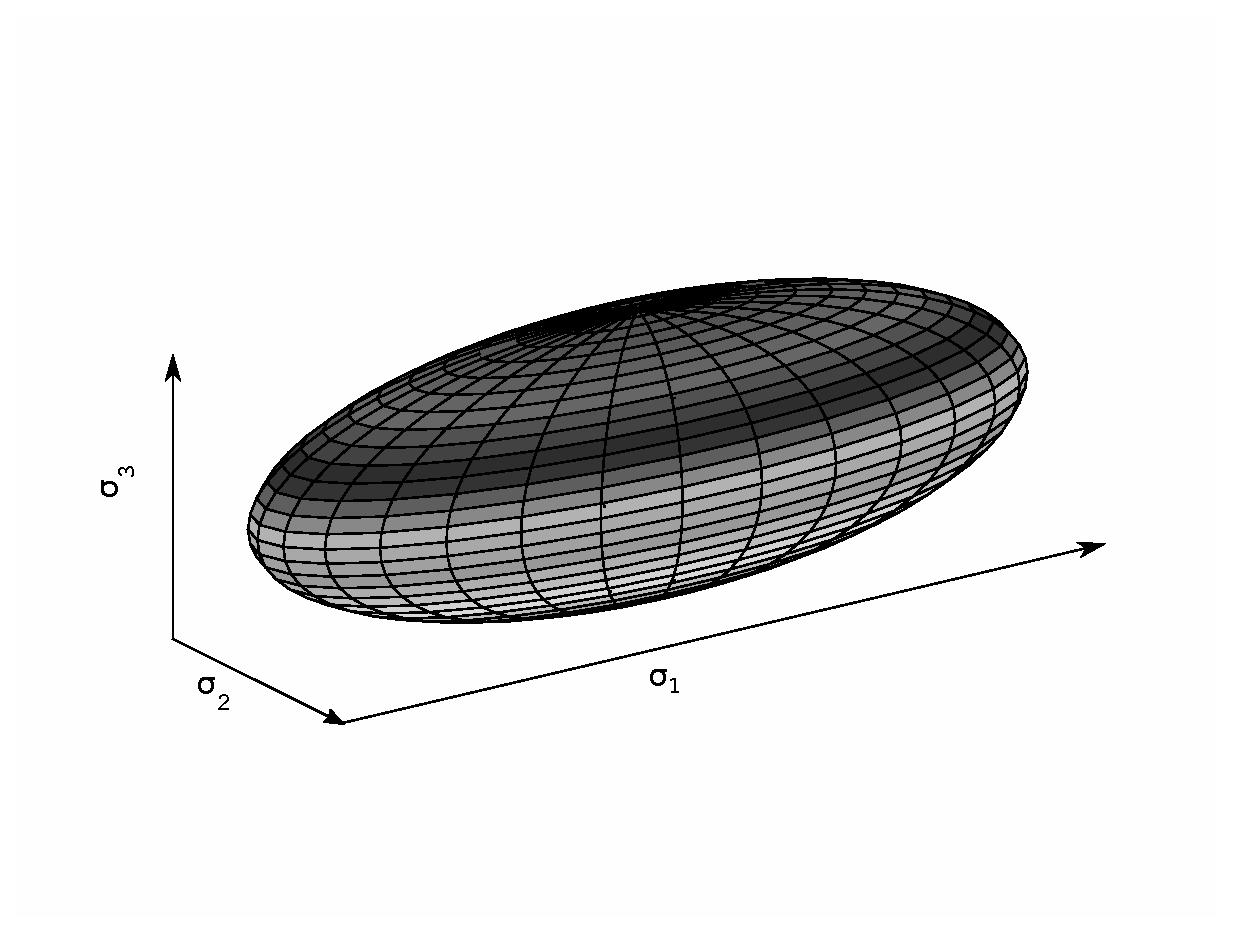
\includegraphics[width=0.7\textwidth]{fig/fmridti/ellipsoid_1.eps}}\\
	\subfloat[The primary, secondary and tertiary Eigen values described in \equationname \ref{eq:dti_ellipsoid}.]{\includegraphics[width=0.7\textwidth]{fig/fmridti/ellipsoid_2.eps}}
	\caption{Visual intuition of the ellipsoid representation of a diffusion tensor voxel.}
	\label{fig:dti_ellipsoid}
\end{figure}

From the raw data, it is possible to determine fractional anisotropy but not the fibre orientation. Diffusion tensor information can also be used to reconstruct white matter bundles in the brain. This technique is termed tractography. Fibre tractography is a very elegant method for delineating individual fibre tracts from diffusion images. Tractography uses diffusion orientation information from tensor imaging to calculate the direction of fibre bundles in-vivo. In deterministic, or streamline tractography, the local tract direction is defined by the major eigenvector of the diffusion tensor \citep{alexander2010deterministic}. This causes issues in voxels with crossing, kissing or splitting fibres. However, as the algorithm is only capable of estimating one fibre orientation \citep{alexander2010deterministic}, probabilistic tractography addresses these issues by estimating the orientations of two or three different fibre populations within a single voxel \citep{behrens2007probabilistic}. Thereafter, at every voxel, the algorithm estimates the most probable fibre orientation and also provides a distribution representing the probability that every other orientation lies along that fibre. This process is repeated many times, each time using a slightly different orientation (according to its likelihood). The integration of all estimates provides a collective measure of connection probability along each tract \citep{behrens2007probabilistic, behrens2003characterization}. \figurename \ref{fig:diff_mri} shows an example of a diffusion MRI image of the human brain.

\begin{figure}
	\centering
	\includegraphics[width=\textwidth]{fig/fmridti/dmri.png}
	\caption{Orientation information from DTI image. Left image shows an axial slice of a single subject's DTI data, registered to structural and MNI standard space. The Right image shows a close-up of the right posterior corpus callosum. Directions corresponding to each colour are as follows: Red - left to right/right to left, green - anterior to posterior/posterior to anterior and blue - superior to inferior/inferior to superior (source \citet{dtiwiki}).}
	\label{fig:diff_mri}
\end{figure}

\section{NeuCube Architecture for Integrating Spatial, Temporal and Orientation Information}

\subsection{Formalisation of the Machine Learning Problem}
The machine learning problem here is to learn a functional mapping of $f(D_{seq}, D_{stat})\rightarrow C$, given a set of training samples  $<D_{seq},D_{stat}, C>$, so that the spatial temporal and orientation information present in $D_{seq}$ and $D_{stat}$ are used to not only increase prediction performance, but also impart robustness to the model. Here $D_{seq}$ and $D_{stat}$ represents the fMRI/EEG and DTI data respectively.

\subsection{NeuCube Personalised SNNc Architecture}
\label{sec:neucube_person}
Here, a personalised SNNc based NeuCube architecture is proposed for the purpose of learning from multi-modal information. The personalised SNNc based NeuCube architecture is a modification of the NeuCube architecture described in Section \ref{sec:neucube_estdm} and depicted in \figurename \ref{fig:neucube_archit}. Before proposing the modified architecture, it is necessary to elaborate certain characteristics of the SNNc in a canonical setting.

\paragraph{Saturation behaviour of canonical NeuCube SNNc:} The classical NeuCube architecture shown in \figurename \ref{fig:neucube_archit} is made up of a single instance of encoder layer, SNNc layer and supervised readout layer. The instances of these layers are initialised before the training process and data is passed through sequentially over time for: (1) Encoding layer to continuously encode the data into spike-timings; (2) SNNc layer to digest the data and update its state; and (3) supervised readout layer to digest the transformed spike-train and create instances in the data space for the K-NN algorithm to act on. NeuCube is a pattern recognition system that learns continuously from data. During the course of development of NeuCube, it is observed that in a vanilla setting, learning continuously from streaming input data has some undesirable effects on the run-time efficiency and performance over time. Upon analysis, it was found this behaviour relates to the single instantiation of the NeuCube SNNc layer. 

To further describe this behaviour, the spike density of SNNc can be defined as the number of neurons that fire at a certain time instance. It is observed that as input data is fed into the SNNc over time, the probability of the neurons in the SNNc firing increases. The spiking neuron of course has a mechanism, such as refractoriness, to avoid continuous spiking; however, over time, periodicity in spike density cannot be avoided. To demonstrate this statement, a set of experiments were conducted using synthetically generated spike data. 

In the experimental setup, a small SNNc was initialised having $27$ neurons. The neurons were spatially distributed in a $3\times 3\time 3$ grid. The network of neurons were connected following the SWC algorithm ($r_{thr}=0.3$). For input data, random input spikes (with spiking probability $0.3$) data $D_{seq}=\{0, 1\}^{200\times 4}$ were synthetically generated for each sample. \tablename \ref{tab:saturation} enlists three instances of the experiment wherein the canonical SNNc unsupervised learning algorithm was run using varying sample sizes and hyperparameter values. At the end of the SNNc simulation, the spike-rate over time (or samples as samples are presented over time) was plotted. It can be observed that irrespective of the hyperparameter settings, a periodicity/total saturation in spike-rate is seen in the SNNc. As a consequence, the spiking patterns after a certain number of sample presentations becomes predictable and does not relate to the variabilities in the sample any more. This fact can be verified from the `sample distance matrix' column where the pairwise hamming distance matrix was plotted across the sample output of the SNNc. The colours (red is high and blue is low) in the plot represents the hamming distance between two samples. It must be noted that the hamming distance between samples not only considers how many times SNNc has spiked for a sample, but also considers when the neurons have spiked. It can be observed there is a lot of variability in the similarity values initially, but as more samples are presented, the spike patterns become more and more similar leading to very small values of dissimilarity. 

The point of including the SNNc layer is to improve pattern formation by expanding it into higher dimensional space. However, the behaviour described above does have a significant impact on pattern generation capabilities of the canonical NeuCube SNNc beyond a certain time. This can be defined as saturation threshold time. There are two directions where research can traipse in order to resolve or further analyse this issue:

\begin{itemize}
	\item Improve the SNNc mechanisms and principles to keep it within sub-threshold limit. In this setting, a single instance of the SNNc can be simulated lifelong without reduction in pattern generation abilities.
	\item Minimise the impact of saturation by using multiple instances of the SNNc and control the sub-threshold state using the hyperparameter values. This approach was used in this work.
\end{itemize}          

\begin{sidewaystable}
	\centering
	\caption{Experimental results showing saturation characteristics of canonical NeuCube SNNc.}
	\label{tab:saturation}
		\begin{tabular}{@{}|l|l|l|l|l|l|l|@{}}
			\toprule \toprule
			\# samples & $v_{thr}$ & $\eta_{thr}$ & $\kappa$ & sample vs spike rate & Hamming distance matrix & saturation type \\ \midrule
			50 & 0.5 & 0 & 0.1 & 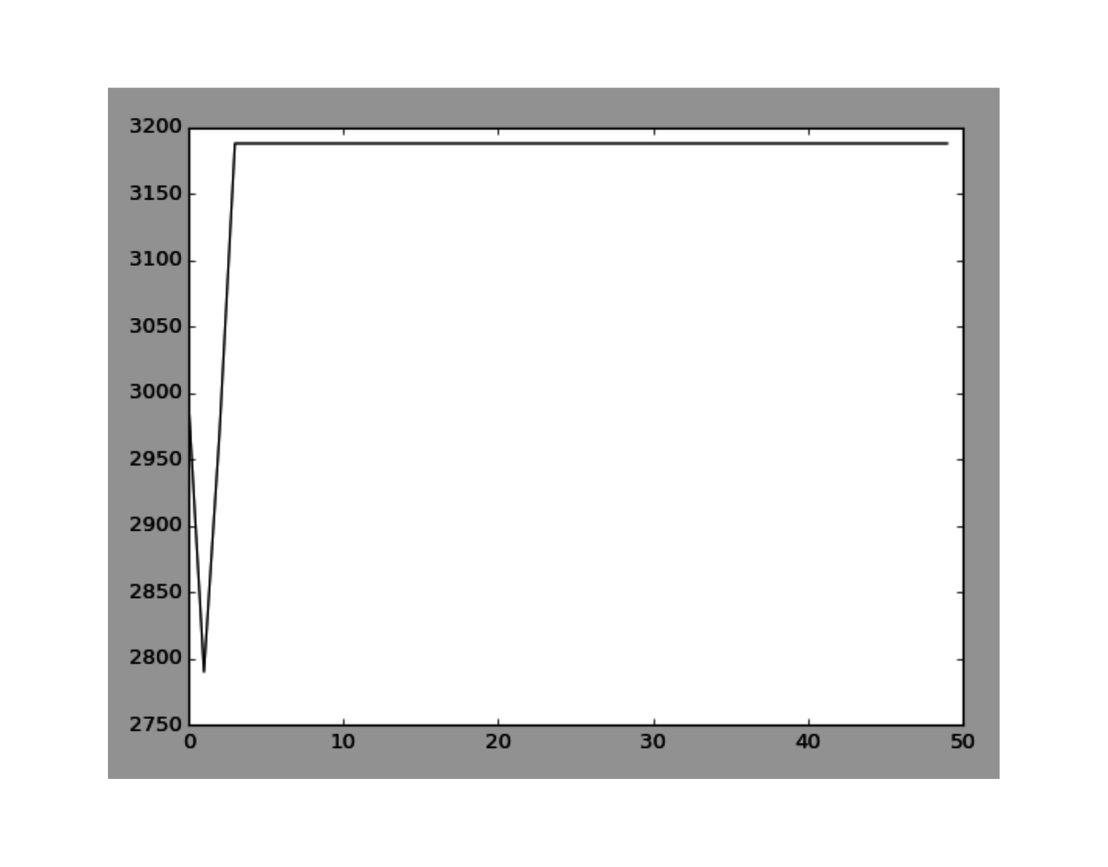
\includegraphics[scale=0.4]{fig/fmridti/sat1.eps}  & 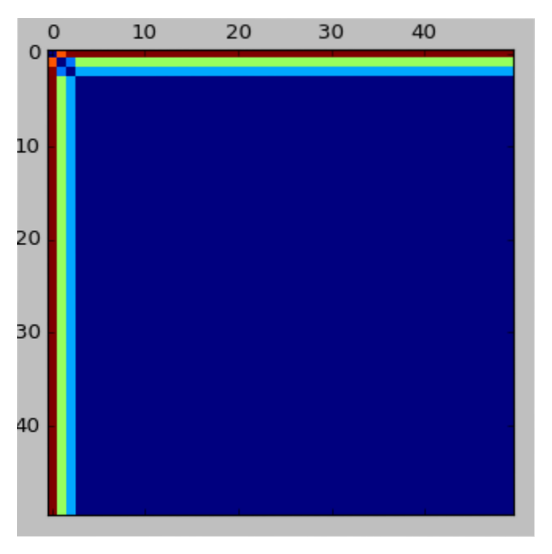
\includegraphics[scale=0.6]{fig/fmridti/sat1d.eps} & total \\ \midrule
			500 & 10 & 0 & 0.1 & 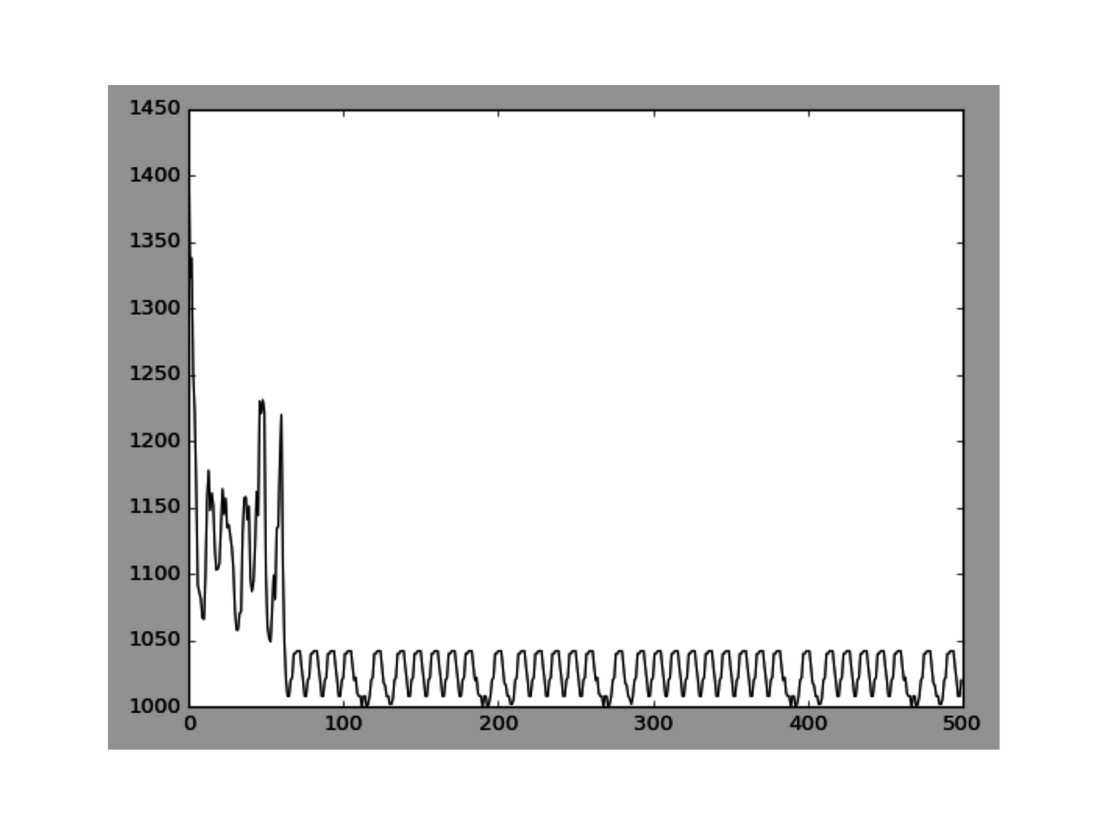
\includegraphics[scale=0.4]{fig/fmridti/sat2.eps} & 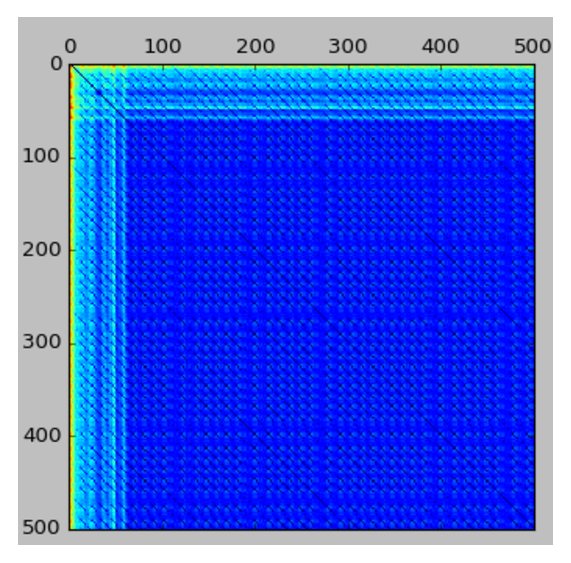
\includegraphics[scale=0.6]{fig/fmridti/sat2d.eps}  & periodic \\ \midrule
			200 & 1 & 15 & 0.1 & 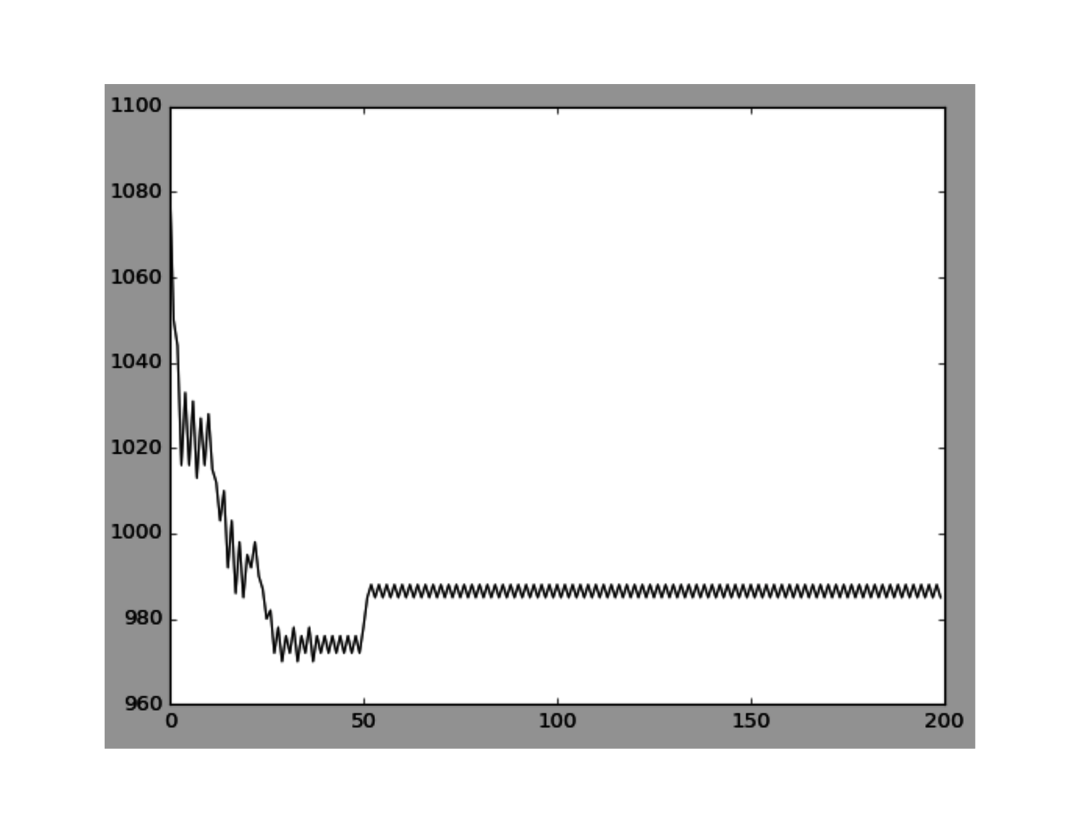
\includegraphics[scale=0.4]{fig/fmridti/sat3.eps} & 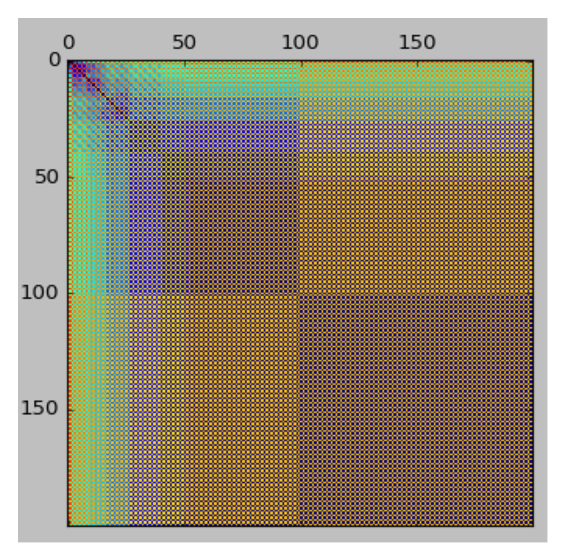
\includegraphics[scale=0.6]{fig/fmridti/sat3d.eps} & periodic \\ \bottomrule \bottomrule
		\end{tabular}%	
\end{sidewaystable}

The personalised SNNc based NeuCube architecture is depicted in \figurename \ref{fig:personaliosed_arch}. In the personalised SNNc approach, usage of multiple instances of SNNc was proposed. In this approach one instance of SNNc is simulated per sample along with a single instance of the encoding layer and supervised readout layer. In this setup, each sample of input data is fed into a unique pre-initialised personal SNNc. The personal SNNc acts as a filter which evolves over time to capture the spatio-temporal relationships within a sample in the synaptic strengths. The knowledge of finite time horizon means the SNNc instance can be kept in a sub-saturation state by controlling the hyperparameter ranges. The other advantage of the personalised SNNc architecture is the ability to avoid the sequential sample presentation bias that may exist if all the samples are fed into a single instance of the SNNc. This means the sequence of the sample presentation does not have any impact on spike patterns generated by the SNNc. The other important aspect of the proposed personalised SNNc architecture is the ability to incorporate multi-modal nature of the input data which will be discussed further.   

\begin{sidewaysfigure}
	\includegraphics[width=0.8\linewidth]{fig/fmridti/neucube_personalised_arch.pdf}
	\caption{Proposed NeuCube personalised SNNc architecture.}
	\label{fig:personaliosed_arch}
\end{sidewaysfigure}


\subsection{Multi-modal Information Integration in SNNc Using Orientation and Spike-time Data}
\label{sec: SNNc}
In this Section, the proposed adaptations of the canonical SNNc unsupervised learning algorithm mentioned earlier in Section \ref{sec:neucube_snnc_learning}, for the purpose of fusing dynamic spatio-temporal and static orientation information from brain data, will be discussed. 

\subsubsection{SNNc Architecture, Mapping and Initialisation}
The SNNc architecture, as described elaborately in Section \ref{subsec:SNNc_init}, are spatially arranged (in three dimensions) set of neurons, partially connected by recurrent synapses forming a directed incomplete and acyclic graph $G=\{M, C, W\}$. The symbols and formalisations are consistent with Chapter \ref{chap:large_snn} unless otherwise stated. The neurons within the network are input or spiking types. The spatial arrangement of the neurons follow a natural ordering and in the case of brain data, integration takes a brain-like shape. The connections of the network are established following the standard SWC \citep{kasabov2014evolving} algorithm.  

\subsubsection{Neuron Dynamics}
The SRM model has been used for implementing the leaky integrate and fire like behaviour of a neuron. The SRM neuron model is used to adapt the membrane potential $v(t)$ of a neuron over time. This neuron model specifies the membrane potential as the sum of: (1) temporal integration of the PSPs and (2) the refractoriness. The PSP kernel $\epsilon_0$ is a function of $t-t^f$, representing the PSP trace over time generated by the firing of neuron $j$ over time. $\tau_m$  is known as the membrane constant which controls the decay rate of the PSP. In the present experiments, a constant $\tau_m = 0.5$ has been used. This means the influence of a pre-synaptic spike diminishes from maximum to minimum within approximately five discrete time intervals. For a more detailed explanation and behaviour of the neuron dynamics, see Section \ref{subsec:SNNc_neuron_model}.

\begin{equation}
\begin{matrix}
\displaystyle v_i(t)=v_{rest}+\sum_{j\in \Tau_i }w_{ji}\sum_{t_j^f\in F_j}\epsilon_0(t-t_j^f)+\eta(t-t_i^f) \\ \\

\epsilon_0(t-t_j^f)=\exp(-\frac{t-t_j^f}{\tau_m})\mathcal{H}(t-t_j^f)\\ \\

\mathcal{H}(t-t_j^f)=\left\{
\begin{array}{@{}cc@{}}
1, & \text{if}\ t-t_j^f\geq 0 \\
0, & \text{otherwise}
\end{array}\right.  \\ \\

\eta(t-t_i)=\left\{
\begin{array}{@{}cc@{}}
-\infty, & \text{if}\ t-t_i^f<\eta_{thr}\\
0, & \text{otherwise}
\end{array}\right.

\end{matrix}
\label{eq:SRM_multimodal_neucube}
\end{equation} 

\paragraph{Python implementation:} The neuron model dynamics has been implemented in python $v3.5$. The neuron model dynamics were implemented as part of the $LeakyIntegrateAndFire$ class shown below. The $simulate()$ method is implemented to simulate the neuron dynamics using the input $spike\_train$ and pre-synaptic connection weights $weight$ and hyperparameter $tau$.
\begin{lstlisting}[language=Python, caption={Python code for NeuCube modified SRM neuron model}]
class LeakyIntegrateAndFireNeuron:
	def __init__(self, predecessor_count, potential_threshold, refractory_threshold, potential_resting, spike_history_length):
		self.predecessor_count = predecessor_count
		self.refractory_threshold = refractory_threshold
		self.potential_threshold = potential_threshold
		self.potential_resting = potential_resting
		self.spike_history_length = spike_history_length
		self.time = 0
		# initialise neuron state
		self.potential = self.potential_resting
		self.refractory_state = 0
		self.potential_state_history = [self.potential]
		self.spike_history = np.zeros((self.spike_history_length, self.predecessor_count), dtype=int)

	@staticmethod
	def spike_response_kernel(current_time, spike_time, tau):
		time_diff = current_time - spike_time
		potential = np.exp(-time_diff / tau)
		return potential

	def simulate(self, spike_train, weight, tau):
		self.time += 1
		self.spike_history = np.delete(self.spike_history, 0, axis=0)
		self.spike_history = np.append(self.spike_history, [spike_train], axis=0)
		current_time = self.spike_history_length
		potential = self.potential
		spike = 0
		if self.refractory_state == 0:
			for k in np.arange(current_time):
				count = np.count_nonzero(self.spike_history[k, :])
				indices = np.nonzero(self.spike_history[k, :])
				for i in range(count):
					w = weight[indices[0][i]]
					potential += w * self.spike_response_kernel(current_time=current_time - 1, spike_time=k, tau=tau)
			self.potential = potential
			self.potential_state_history.append(self.potential)
			if self.potential > self.potential_threshold:
				self.refractory_state = self.refractory_threshold
				self.potential = self.potential_resting
				spike = 1
		else:
			self.refractory_state = max(0, self.refractory_state - 1)
			self.potential = max(self.potential_resting, self.potential)
			self.potential_state_history.append(self.potential)
	return spike
	
\end{lstlisting}

\subsubsection{Adaptation of Synaptic Strengths of the SNNc}
\label{subsec:SNNc_learning}
The unsupervised learning algorithm in the SNNc is the most important aspect of the proposed architecture for integrating multi-modal information. In a neural network paradigm, learning is achieved through the synaptic strength updates of the network. The learning behaviour of the SNNc can be explained using the learning model of a single spiking neuron. Considering the single neuron architecture, as shown in \figurename \ref{fig:neuron_architecture}, the unsupervised learning problem is the a scheme of updating the $w_{ji}$'s by $\Delta w_{ji}(t)$ over the simulation time $T$. In a recurrent SNNc layer, the aim is to learn dynamic influence from dynamic data (fMRI) and static orientation influence from static data (DTI).  


\subsubsection{Dynamic Influence from fMRI/EEG}
\label{subsec:phi}

In the majority of the machine learning applications, models are trained on static data, where a sample is represented by a vector of numbers $\mathbf{d}=\{d_1,d_2,\cdots\}$, where each of the elements within the tuple $d$ represents the scalar value of a particular feature. However, in this case with fMRI or EEG data, a sample is represented by a matrix $\mathbf{D_{seq}=\{d_1, d_2,\cdots, d_n\}}$, where $\mathbf{d_i}=\{d_i(1), d_i(2),\cdots d_i(t)\}$. The sample representation is not only multidimensional but also is ordered in time (sequence). Learning from these types of data in machine learning is known as sequence learning and techniques, like the hidden Markov model and flavours of recurrent neural network have shown promise in learning from such sequences. In this instance, an unsupervised sequence learning algorithm will be described that is within the NeuCube SNNc layer and utilises the sequential information as part of its learning mechanism. The sequential information within the SNNc architecture is named as the dynamic influence and is denoted by $\phi$.        

The dynamic influence from the spike-time data using the STDP learning algorithm was modelled. As discussed elaborately in Section \ref{subsec:STDP}, STDP is a temporally asynchronous form of Hebbian learning ("neurons wire together, if they fire together") \citep{hebb1949organization} induced by the temporal correlation of the spikes. Due to the online nature of the learning within the SNNc layer, the canonical online formulation of the STDP learning rule have been used. \citet{sjostrom2010spike} proposed the on-line STDP update rule by modifying the canonical STDP rule. In the on-line setting, the $\phi_{ji}$ is calculated every time a neuron $i$ fires a spike or receives a spike from neuron $j$. \equationname \ref{eq:multimodal_stdp_online} formalises the weight update rule that was used to calculate the dynamic influence. The first term in the right hand side of \equationname \ref{eq:stdp_online} corresponds to the LTP update and is calculated when neuron $i$ fires a spike at time $t$. The second term is the LTD update and is calculated when neuron $i$ receives a spike from neuron $j$ at time $t$. 


\begin{equation}
\phi_{ji}(t) = \sum_f \kappa_+\exp(-(t-t_j^f))-\sum_g \kappa_- \exp(-(t-t_i^g))
\label{eq:multimodal_stdp_online}
\end{equation}

\paragraph{Python implementation:} The python implementation of \equationname \ref{eq:multimodal_stdp_online} is given below. The $STDP()$ method takes the pre- and post-synaptic spike history $t_j^f$s and $t_i^g$s along with the learning rate hyperparameter $\kappa$ to generate the dynamic influence $phi$. 

\begin{lstlisting}[language=Python, caption={Python code for calculating dynamic influence}, label={list:stdp}]
def STDP(pre_synaptic_spike_history, post_synaptic_spike_history, kappa):	
	assert isinstance(pre_synaptic_spike_history, list)
	assert isinstance(post_synaptic_spike_history, list)
	if len(pre_synaptic_spike_history) != len(post_synaptic_spike_history):
	raise ValueError("Length mismatch of pre and post synaptic spike history!!")
	pre_synaptic_spike_energy = 0
	post_synaptic_spike_energy = 0
	importance_of_LTP = 0.3
	importance_of_LTD = 0.3
	time_history = len(pre_synaptic_spike_history)
	pre_synaptic_spike_history = np.asarray(pre_synaptic_spike_history)
	post_synaptic_spike_history = np.asarray(post_synaptic_spike_history)
	"""
	calculation of LTD
	"""
	if pre_synaptic_spike_history[time_history - 1] == 1:
		post_spike_indices = np.nonzero(post_synaptic_spike_history)[0]
		k = kappa * np.exp(-(1 - importance_of_LTD) * ((time_history - 1) - post_spike_indices))
		pre_synaptic_spike_energy = np.sum(k)
	
	"""
	calculation of LTP
	"""
	if post_synaptic_spike_history[time_history - 1] == 1:
		pre_spike_indices = np.nonzero(pre_synaptic_spike_history)[0]
		k = kappa * np.exp(-(1 - importance_of_LTP) * ((time_history - 1) - pre_spike_indices))
		post_synaptic_spike_energy = np.sum(k)
	phi = post_synaptic_spike_energy - pre_synaptic_spike_energy
	return phi
\end{lstlisting}


\begin{figure}
	\centering
	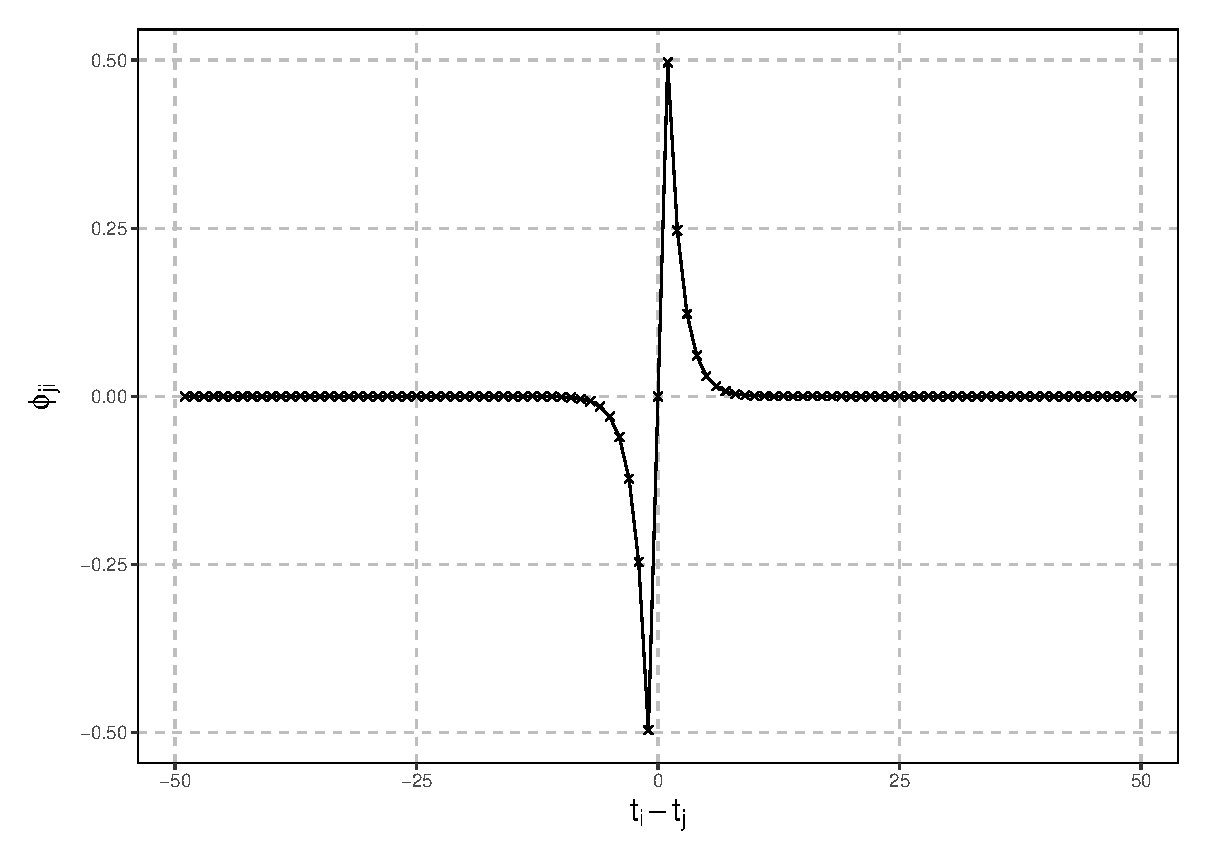
\includegraphics[width=\linewidth]{fig/fmridti/STDP.eps}
	\caption{Plot of the STDP weight update as a function of the relative time difference of the pre and post synaptic spikes. The data for this plot was generated using code snippet \ref{list:stdp} with hyperparameter $\kappa_+=\kappa_-=0.5$.}
	\label{fig:stdp}
\end{figure}



\subsubsection{Static Orientation Influence from DTI Tractography Data}

The present study has used the DTI data in the form of orientation vectors representing mean orientation of the fibre tract at different voxel locations. The process of generating the orientation data from a DTI image is described later in Section \ref{subsec:schizophrenia_method}. The orientation vector of a sample DTI image is represented by a matrix $\mathbf{D_{stat}} \in \mathbb{R}^{|N|\times 3}$, where each feature/voxel is made up of a 3D vector describing the primary orientation of the fibre in the Cartesian coordinate system.   
\begin{figure}
	\centering
	\includegraphics[width=\linewidth]{fig/fmridti/angular_influence.png}
	\caption{Example of a pre-synaptic neuron $j$ connected to two post synaptic neurons $i_1$ and $i_2$. Each neurons spatial location is defined by the polar coordinates $(r, \alpha$).}
	\label{fig:ang_inf}
\end{figure}

Here, the interest lies in establishing a learning rule that does not only utilises dynamic data influence as described in Section \ref{subsec:phi}, but can also make use of the static orientation influence from the DTI data. The intuition behind the orientation influence can be explained again by a small SNNc architecture consisting of three neurons as shown in \figurename \ref{fig:ang_inf}. The figure shows a single pre-synaptic neuron $j$ connected to two post synaptic neurons $i_1$ and $i_2$. The important aspect to note here is that the neurons in this diagram have spatial allocations contrary to the one in \figurename \ref{fig:neuron_architecture}. The location of the neurons are defined by the radial and the angular coordinates in the polar coordinate system. Now, the intent is to measure the orientation influence $\psi$ of neuron $j$ on neurons $\{i_1, i_2\}$. The neuron $j$ will be referred to as the pivot neuron. The orientation vector of the pivot neuron (from DTI data) is be represented by $(r_j, \alpha_j)$. The orientation influence of the pivot neuron on the post-synaptic neurons $\{i_1,i_2\}$ is defined by the angular proximity of the pivot neuron's DTI orientation vector to the synaptic orientations of the neuron pairs.  In that way, as per the hypothesis, the pivot neuron wields a stronger angular influence on the neurons that lie in closer angular proximity to the orientation vector of the pivot neuron. Therefore in \figurename \ref{fig:ang_inf}, the orientation influence of neuron $j$ can be arranged as $i_1>i_2$ due to the angular proximity of $i_1$ and $j$ being greater than $i_2$ and $j$. 

Even though a 2D vector space has been used for explaining the intuition of angular influence, the SNNc neurons reside in a 3D space. The intuition can be extended to the 3D vector space by adding another dimension in the coordinate system. In 3D, the spherical coordinates of a point are given by $(r,\alpha, \beta)$, where $r$ is the scalar distance of the point from the centre, $\alpha$ and $\beta$ are the elevation and azimuth angle from the centre. A Gaussian radial basis (GRB) kernel has been utilised to realise the elevation and azimuth orientation influences given the elevation and azimuth data of the neurons. $\psi$ is calculated as the mean of azimuth and elevation influences between pre- and post-synaptic neurons $j$ and $i$ according to \equationname \ref{eq:angular_influence}.

\begin{equation}
\begin{matrix}
\psi_{ji}=\frac{\psi_{ji}^\alpha+\psi_{ji}^\beta}{2} \\ \\

\psi_{ji}^\alpha=\exp(\frac{||\alpha_{ji}-\alpha_j^{dti}||^2}{2\gamma^2})\\ \\

\psi_{ji}^\beta=\exp(\frac{||\beta_{ji}-\beta_j^{dti}||^2}{2\gamma^2})

\end{matrix}
\label{eq:angular_influence}
\end{equation} 

\paragraph{Python implementation:} The python implementation of \equationname \ref{eq:angular_influence} is given below. The $angular\_influence()$ method takes the coordinates of two neurons and the orientation information, and outputs the orientation influence $psi$. 

\begin{lstlisting}[language=Python, caption={Python code for calculating static orientation influence}]
def angular_influence(pivot_coordinate, sphere_coordinate, elevation_angle, azimuth_angle):
	assert isinstance(pivot_coordinate, np.ndarray)
	assert isinstance(sphere_coordinate, np.ndarray)
	assert isinstance(elevation_angle, float)
	assert isinstance(azimuth_angle, float)
	
	standard_deviation = 8	
	relative_sphere_coordinate = np.subtract(sphere_coordinate, pivot_coordinate)
	radius, elevation, azimuth = cart2sph(relative_sphere_coordinate[0], relative_sphere_coordinate[1], relative_sphere_coordinate[2])	
	el_prob = radial_decay(elevation, elevation_angle, standard_deviation)
	az_prob = radial_decay(azimuth, azimuth_angle, standard_deviation)
	psi = (el_prob + az_prob) / 2
	return psi
	
def cart2sph(x, y, z):
	radius = math.sqrt(x ** 2 + y ** 2 + z ** 2)
	elevation = math.atan2(math.sqrt(x ** 2 + y ** 2), z)
	azimuth = math.atan2(y, z)	
	elevation *= 180 / math.pi
	azimuth *= 180 / math.pi
	return (radius, elevation, azimuth)

def radial_decay(x, mu, sigma):
	return math.exp(-1 * (x - mu) ** 2 / (2 * sigma ** 2))
\end{lstlisting}

\begin{figure}
	\centering
	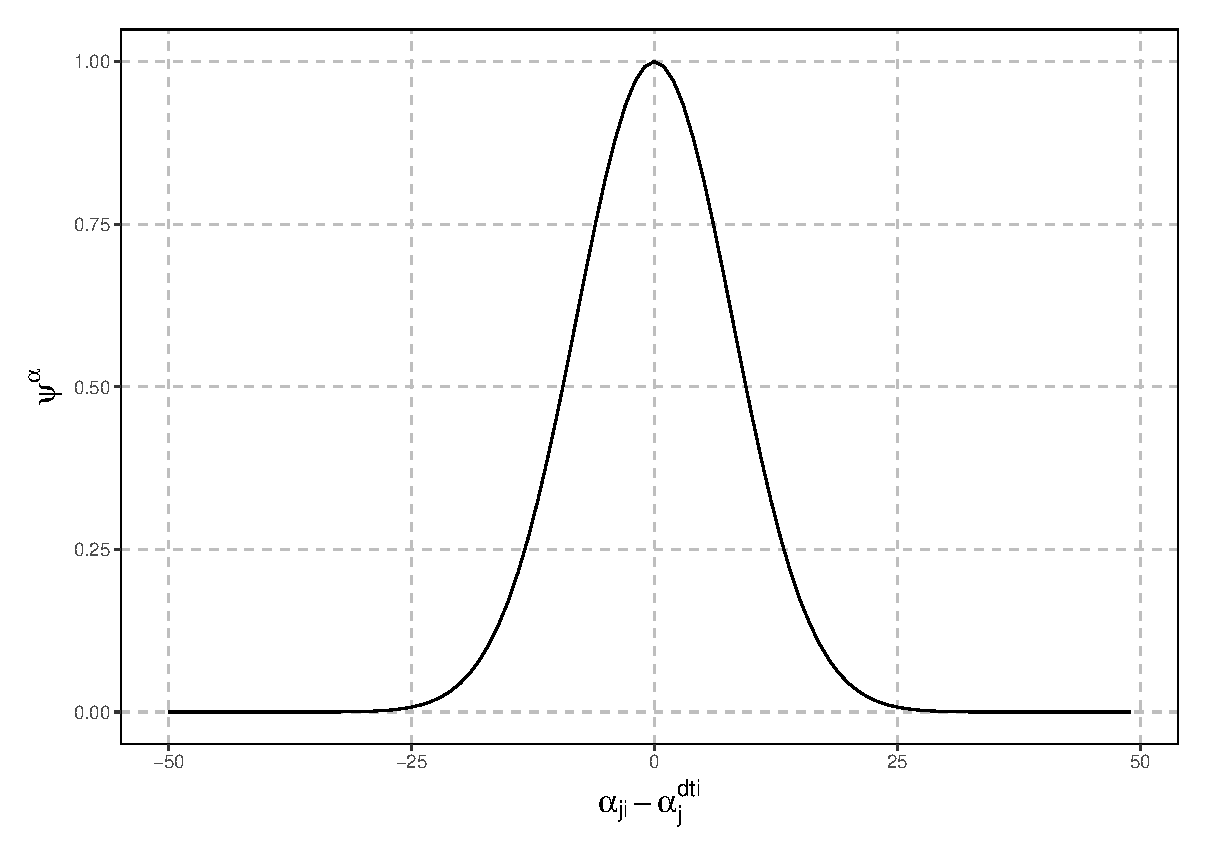
\includegraphics[width=\linewidth]{fig/fmridti/angular_influence_rbf.eps}
	\caption{Plot of the elevation influence $\psi^\alpha$ as a function of the radial distance $\alpha_{ji}-\alpha_j^{dti}$ and $\gamma=8$.}
	\label{fig:angular_influence_rbf}
\end{figure}

The GRB kernels exponentially decay the orientation influence as the Euclidean norm $||\alpha_{ji}-\alpha_j||$ and $||\beta_{ji}-\beta_j||$ increases. The variance hyperparameter $\gamma^2$ controls the speed with which the orientation influence decays with increasing radial distance (see \figurename \ref{fig:angular_influence_rbf}). The overall orientation influence is calculated as the mean of the elevation and azimuth influence, as shown in \equationname \ref{eq:angular_influence}.  

\subsection{Orientation Influence Driven STDP (oiSTDP) Learning in SNNc}
\begin{algorithm}
	\begin{algorithmic}[1]
		\STATE input: $G=\{M,C,W\}$, $D_{seq}\in \{0, 1\}^{|N|\times |T|}$, $D_{stat}\in \mathbb{R}^{|N|\times 3}$, $loc \in \mathbb{R}^{|M|\times 3}$,$\{hyperparameters=v_{thr}, \eta_{thr}, \kappa\}$
		\STATE output: $O_{seq} \in \{0, 1\}^{|M|\times |T|}$
		\STATE $O_{seq}[N,T]\leftarrow D_{seq}$
		\FOR{$t \in T$}
			\STATE initialise $C_{learn}\leftarrow \{\}$
			\FOR{$i$ in spiking neurons $Q$}
				\STATE find firing(at time $t-1$) pre-synaptic neurons, $J^{spk(t)}_i$
				\STATE set $C^{ltd}_i \leftarrow(J^{spk}_i, i)$
				\STATE $C_{learn}+\leftarrow C^{ltd}_i$
				\STATE simulate $i$ as per \equationname \ref{eq:SRM_neucube}
				\IF{$i$ fires a spike}
					\STATE $O_{seq}[i,t+1]\leftarrow 1$	
					\STATE find pre-synaptic neurons, $J_{i}$
					\STATE set $C_i^{ltp}\leftarrow(J_i,i)$
					\STATE set $C_{learn}+\leftarrow C^{ltp}_i$
				\ENDIF
		\ENDFOR
		\FOR{$c_{ji}$ in $C_{learn}$ }
			\STATE initialise $\psi_{ji}\leftarrow 1$
			\IF{$j$ in $N$}
				\STATE $(r_j^{dti}, \alpha_j^{dti},\beta_j^{dti})\leftarrow cart2sph(D_{stat}[j])$
				\STATE $(r_{ji},\alpha_{ji},\beta_{ji})\leftarrow cart2sph(loc[i]-loc[j])$
				\STATE calculate $\psi_{ji}$ as per \equationname \ref{eq:angular_influence}	
			\ENDIF
			\STATE calculate $\phi_{ji}$ as per Eq. \ref{eq:stdp_online}
			\STATE set $\Delta w_{ji}\leftarrow \psi_{ji}\cdot \phi_{ji}$
			\STATE update $w_{ji}\leftarrow w_{ji}+\Delta w$
		\ENDFOR
		\ENDFOR
		
	\end{algorithmic}
	\caption{oiSTDP-based SNNc learning algorithm}
	\label{alg:oiSTDP}
\end{algorithm}
\algorithmname \ref{alg:oiSTDP} describes the oiSTDP learning algorithm step by step. The unsupervised learning is executed on a preinitialised SNNc. The algorithm takes: (1) the dynamic data $D_{seq}$ (fMRI/EEG) in the form of spikes; (2) the static orientation data $D_{stat}$ as 3D orientation vectors; and (3) the coordinates of the SNNc neurons as the input. The output of the learning algorithm are the spikes in the higher dimensional space in the form of $O_{seq}$. Over simulation time $T$, the execution of the algorithm can be divided into two sequential blocks:
\begin{enumerate}
	\item Block 1 (line 6 to 17): First, each spiking neuron in set $Q$ is queried for the pre-synaptic neurons $J_i^{spk}$, that has fired a spike at time $t$ . These connections are stored in $C_{learn}$ for later updating the weights as per the LTD rule. Then the spiking neuron is simulated to update the membrane potential. If the neuron spikes as a result of neuron simulation (line 10), a spike is added to $O_{seq}$ and the pre-synaptic connections are again added to the variable $C_{learn}$ for later weight update as per the LTP rule.
	\item Block 2 (line 18 to 28): This block implements the weight update rule. At every time iteration $t$, synaptic strengths are updated for all the connections stored in $C_{learn}$. Lines 20 to 24 are the steps for calculating the orientation influence $\psi$. The function $cart2sph(.)$ takes a 3D Cartesian coordinate ($x, y, z$) as input and outputs the spherical coordinate ($r,\alpha, \beta$). The following formulae are used for this conversion:\\
	$\displaystyle r=\sqrt{x^2+y^2+z^2}$\\ $\alpha=\tan^{-1} \frac{\sqrt{x^2+y^2}}{z}$\\$\beta=\tan^{-1}\frac{y}{z}$\\
	The weight update $\Delta w_{ji}$ for connection $C_{ji}$ is the product of $\psi_{ji}$ and $\phi_{ji}$ (line 27). In this way, the orientation influence has been used as a modulation factor of the dynamic influence. $phi$ and $psi$ are bound to $[-1, 1]$ and $[0, 1]$ respectively. Henceforth, $Delta w$ is bound between $[-1, 1]$. The most important characteristic of this learning rule is, of course, the inclusion of the orientation influence along with the dynamic influence in the weight update rule formulation. The rationale behind this formulation is to bind the coincidence (STDP) and tract information together in a way such that the strongest weight update occurs between a neuron pair when (1) there is maximal coincidence between the pre-synaptic and post-synaptic firing, and (2) the orientation of a neuron pair matches the DTI orientation data of the pre-synaptic neuron. Hence, the relations observed in the synaptic strengths of the SNNc network are representative of both the spatio-temporal coincidence generated from the encoded spike sequence and the orientation information produced by the DTI data. In this way, the spatial, temporal and orientation information in the synaptic strengths are able to be captured. \figurename \ref{fig:aiSTDP_graph} shows the behaviour of the oiSTDP update rule. The X and Y axes are the radial orientation distance between the neuron pair and the temporal difference between the pre and post-synaptic firing times, respectively. The figure shows a mirrored inverted half Mexican hat behaviour. It is visible that every slice across $r_{ji}$ axis mimics the STDP behaviour shown in \figurename \ref{fig:stdp}.  The top half of the Mexican hat relates to the positive LTP weight update, which peaks at the minimum angular distance and decays with increasing angular distance. The bottom inverse half, on the contrary, relates to negative LTD weight update which achieves a negative peak at the minimum angular distance. In this way, the angular proximity of the neurons plays a role in modulating the spike synchronicity driven dynamic influence.   	 
\end{enumerate}   
\begin{figure}
	\centering
	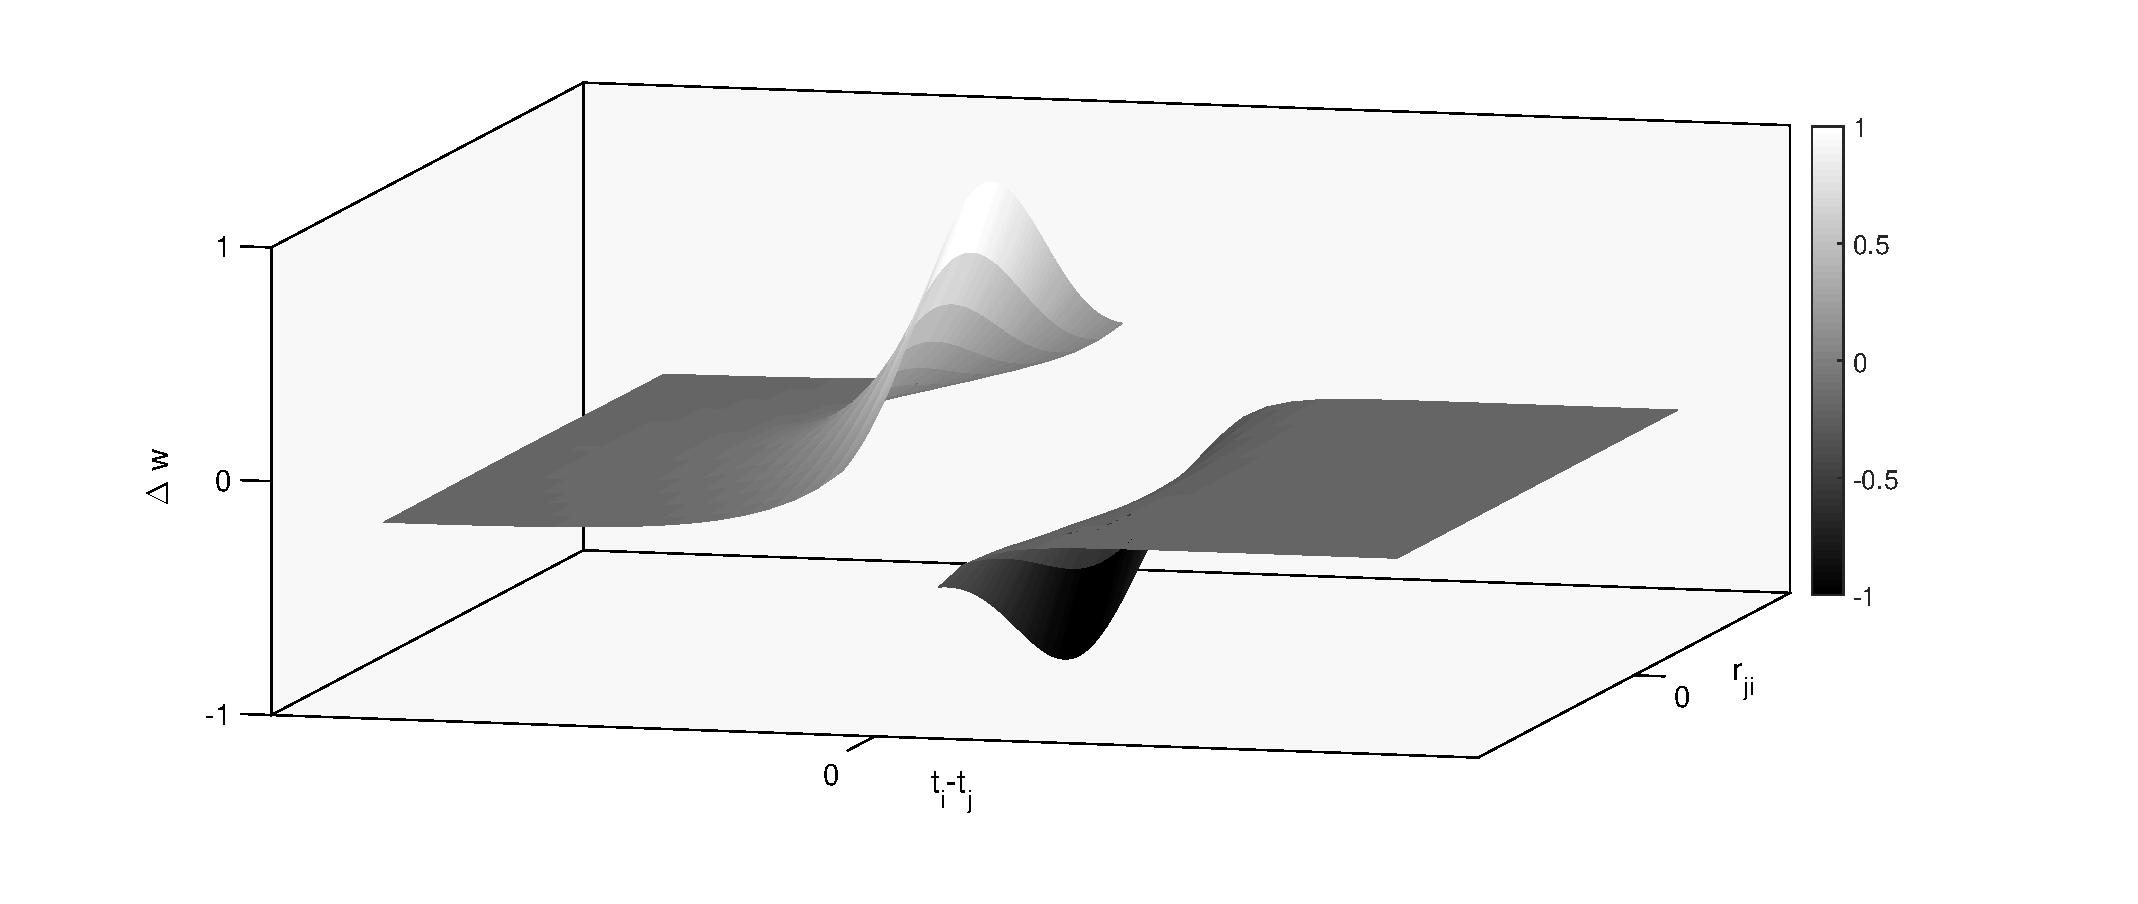
\includegraphics[width=\linewidth]{fig/fmridti/aiSTDP.eps}
	\caption{Graph showing the relationship of oiSTDP weight update $\Delta w$ with post and pre synaptic firing time difference $t_i-t_j$ and orientation distance $r_{ji}$. As the temporal difference between neuronal spikes decreases, the effect on weight updating increases, so that spikes timed closely together lead to greater increases in weight updating than spikes timed further apart. The order of spikes also affects weight updating. If neuron $j$ fires before neuron $i$ consistently, then the synaptic weight between them continues to increase; however, if the order switches, the weight is reduced.}
	\label{fig:aiSTDP_graph}
\end{figure}

\section{Analysis of oiSTDP Algorithm Using Synthetic Data}
\label{subsec:synthetic}
\begin{sidewaysfigure}
	\centering
	\subfloat[3D view]{\label{ex00}
		\includegraphics[scale=0.12]{fig/fmridti/zerozero3d.eps}}
	\subfloat[Horizontal view (X Y plane)]{\label{ex0}
		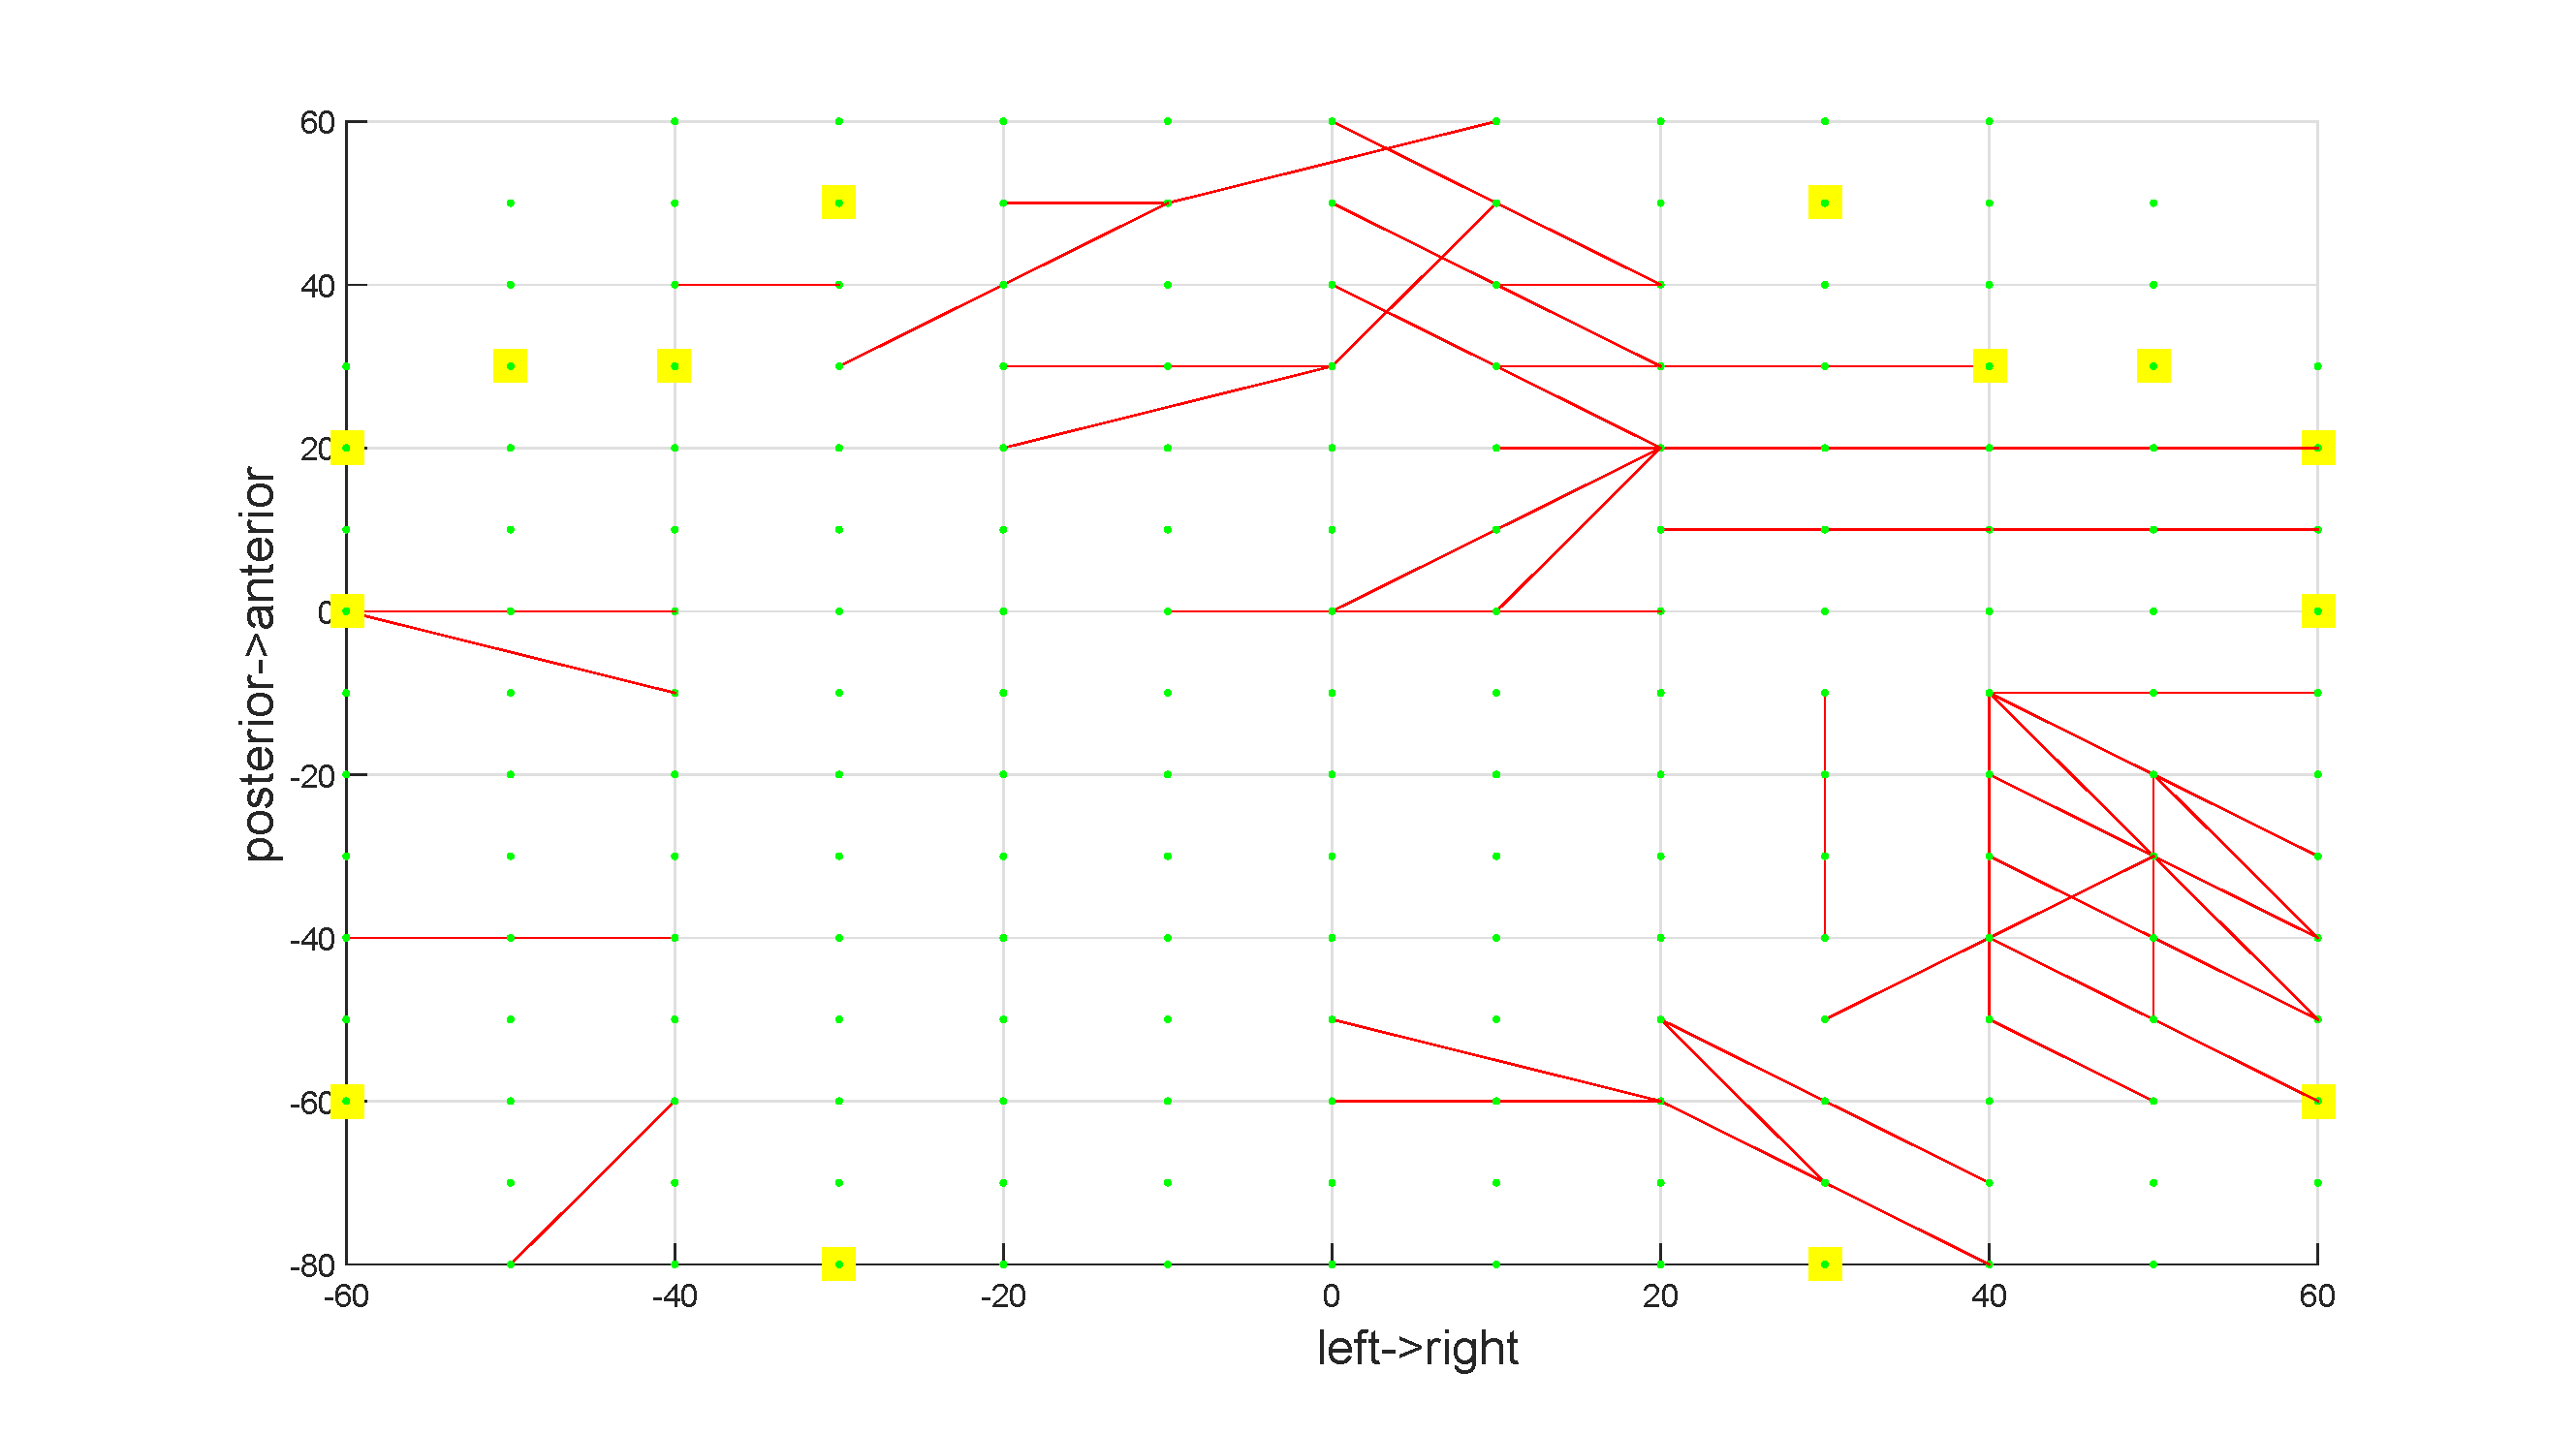
\includegraphics[scale=0.12]{fig/fmridti/zerozeroxy.eps}}
	\subfloat[Coronal view (X Z plane)]{\label{ex1}
		\includegraphics[scale=0.12]{fig/fmridti/zerozeroxz.eps}}\\
	
	\subfloat[3D view]{\label{ex03}
		\includegraphics[scale=0.12]{fig/fmridti/ff3d.eps}}
	\subfloat[Horizontal view]{\label{ex3}
		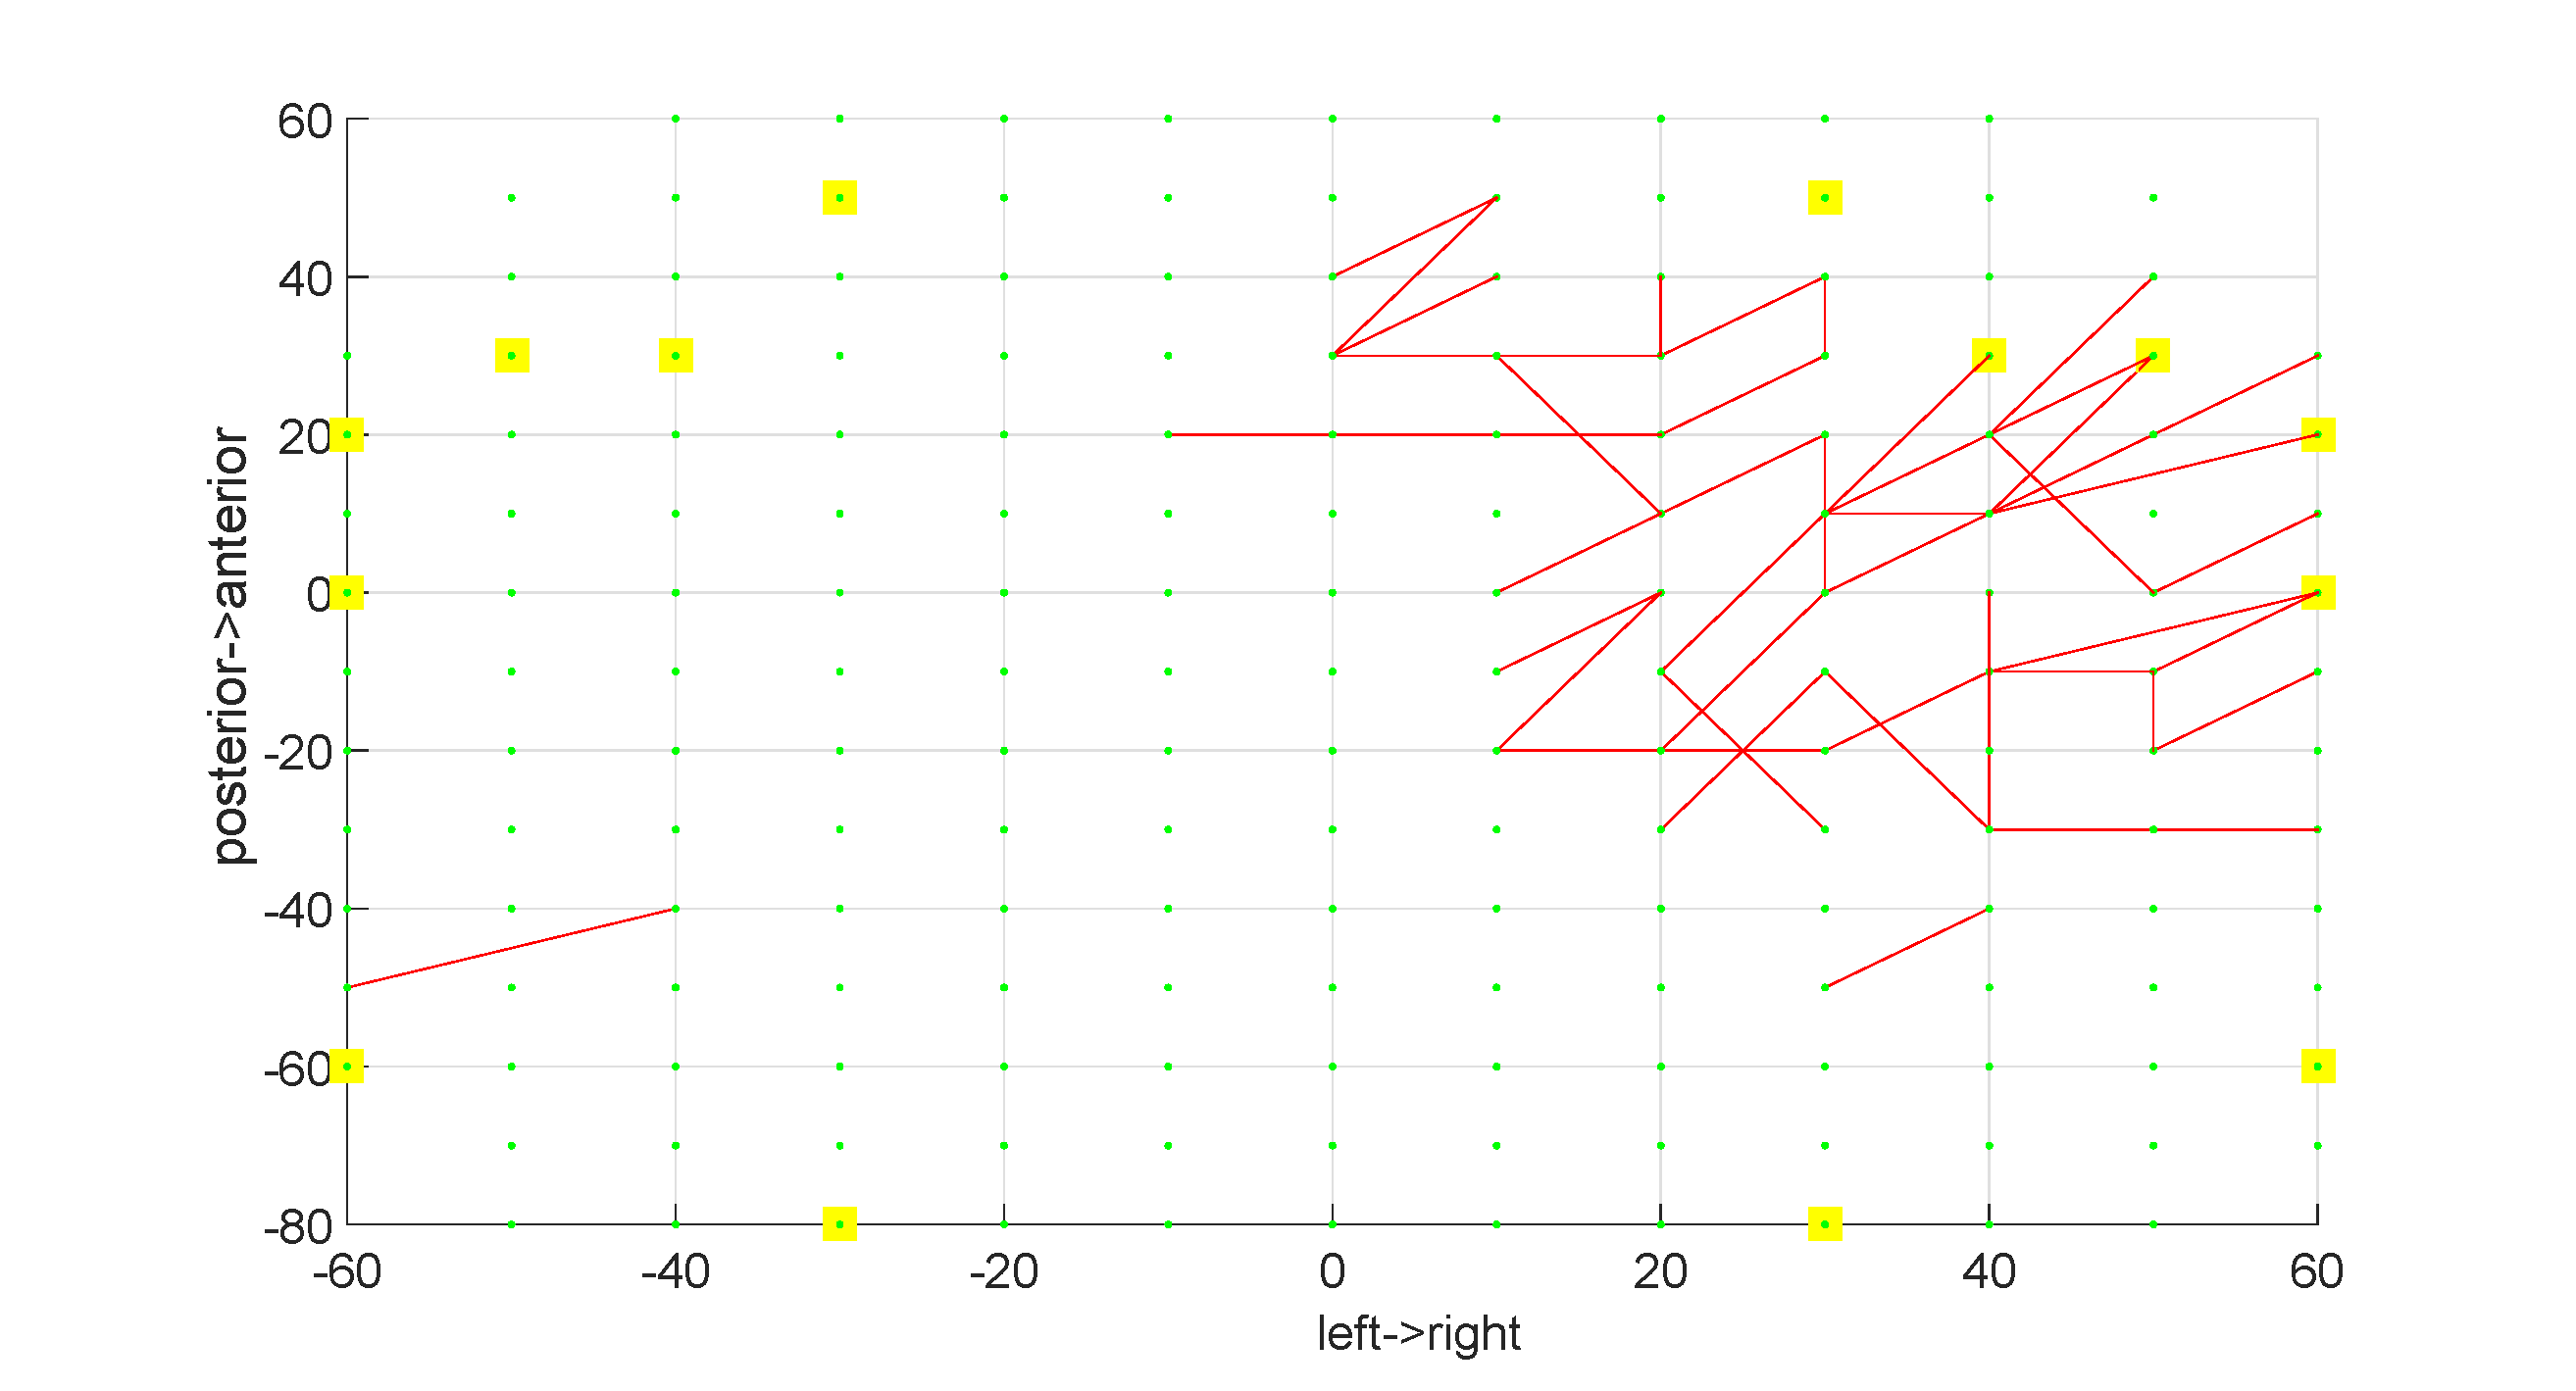
\includegraphics[scale=0.12]{fig/fmridti/ffxy.eps}}
	\subfloat[Coronal view]{\label{ex4}
		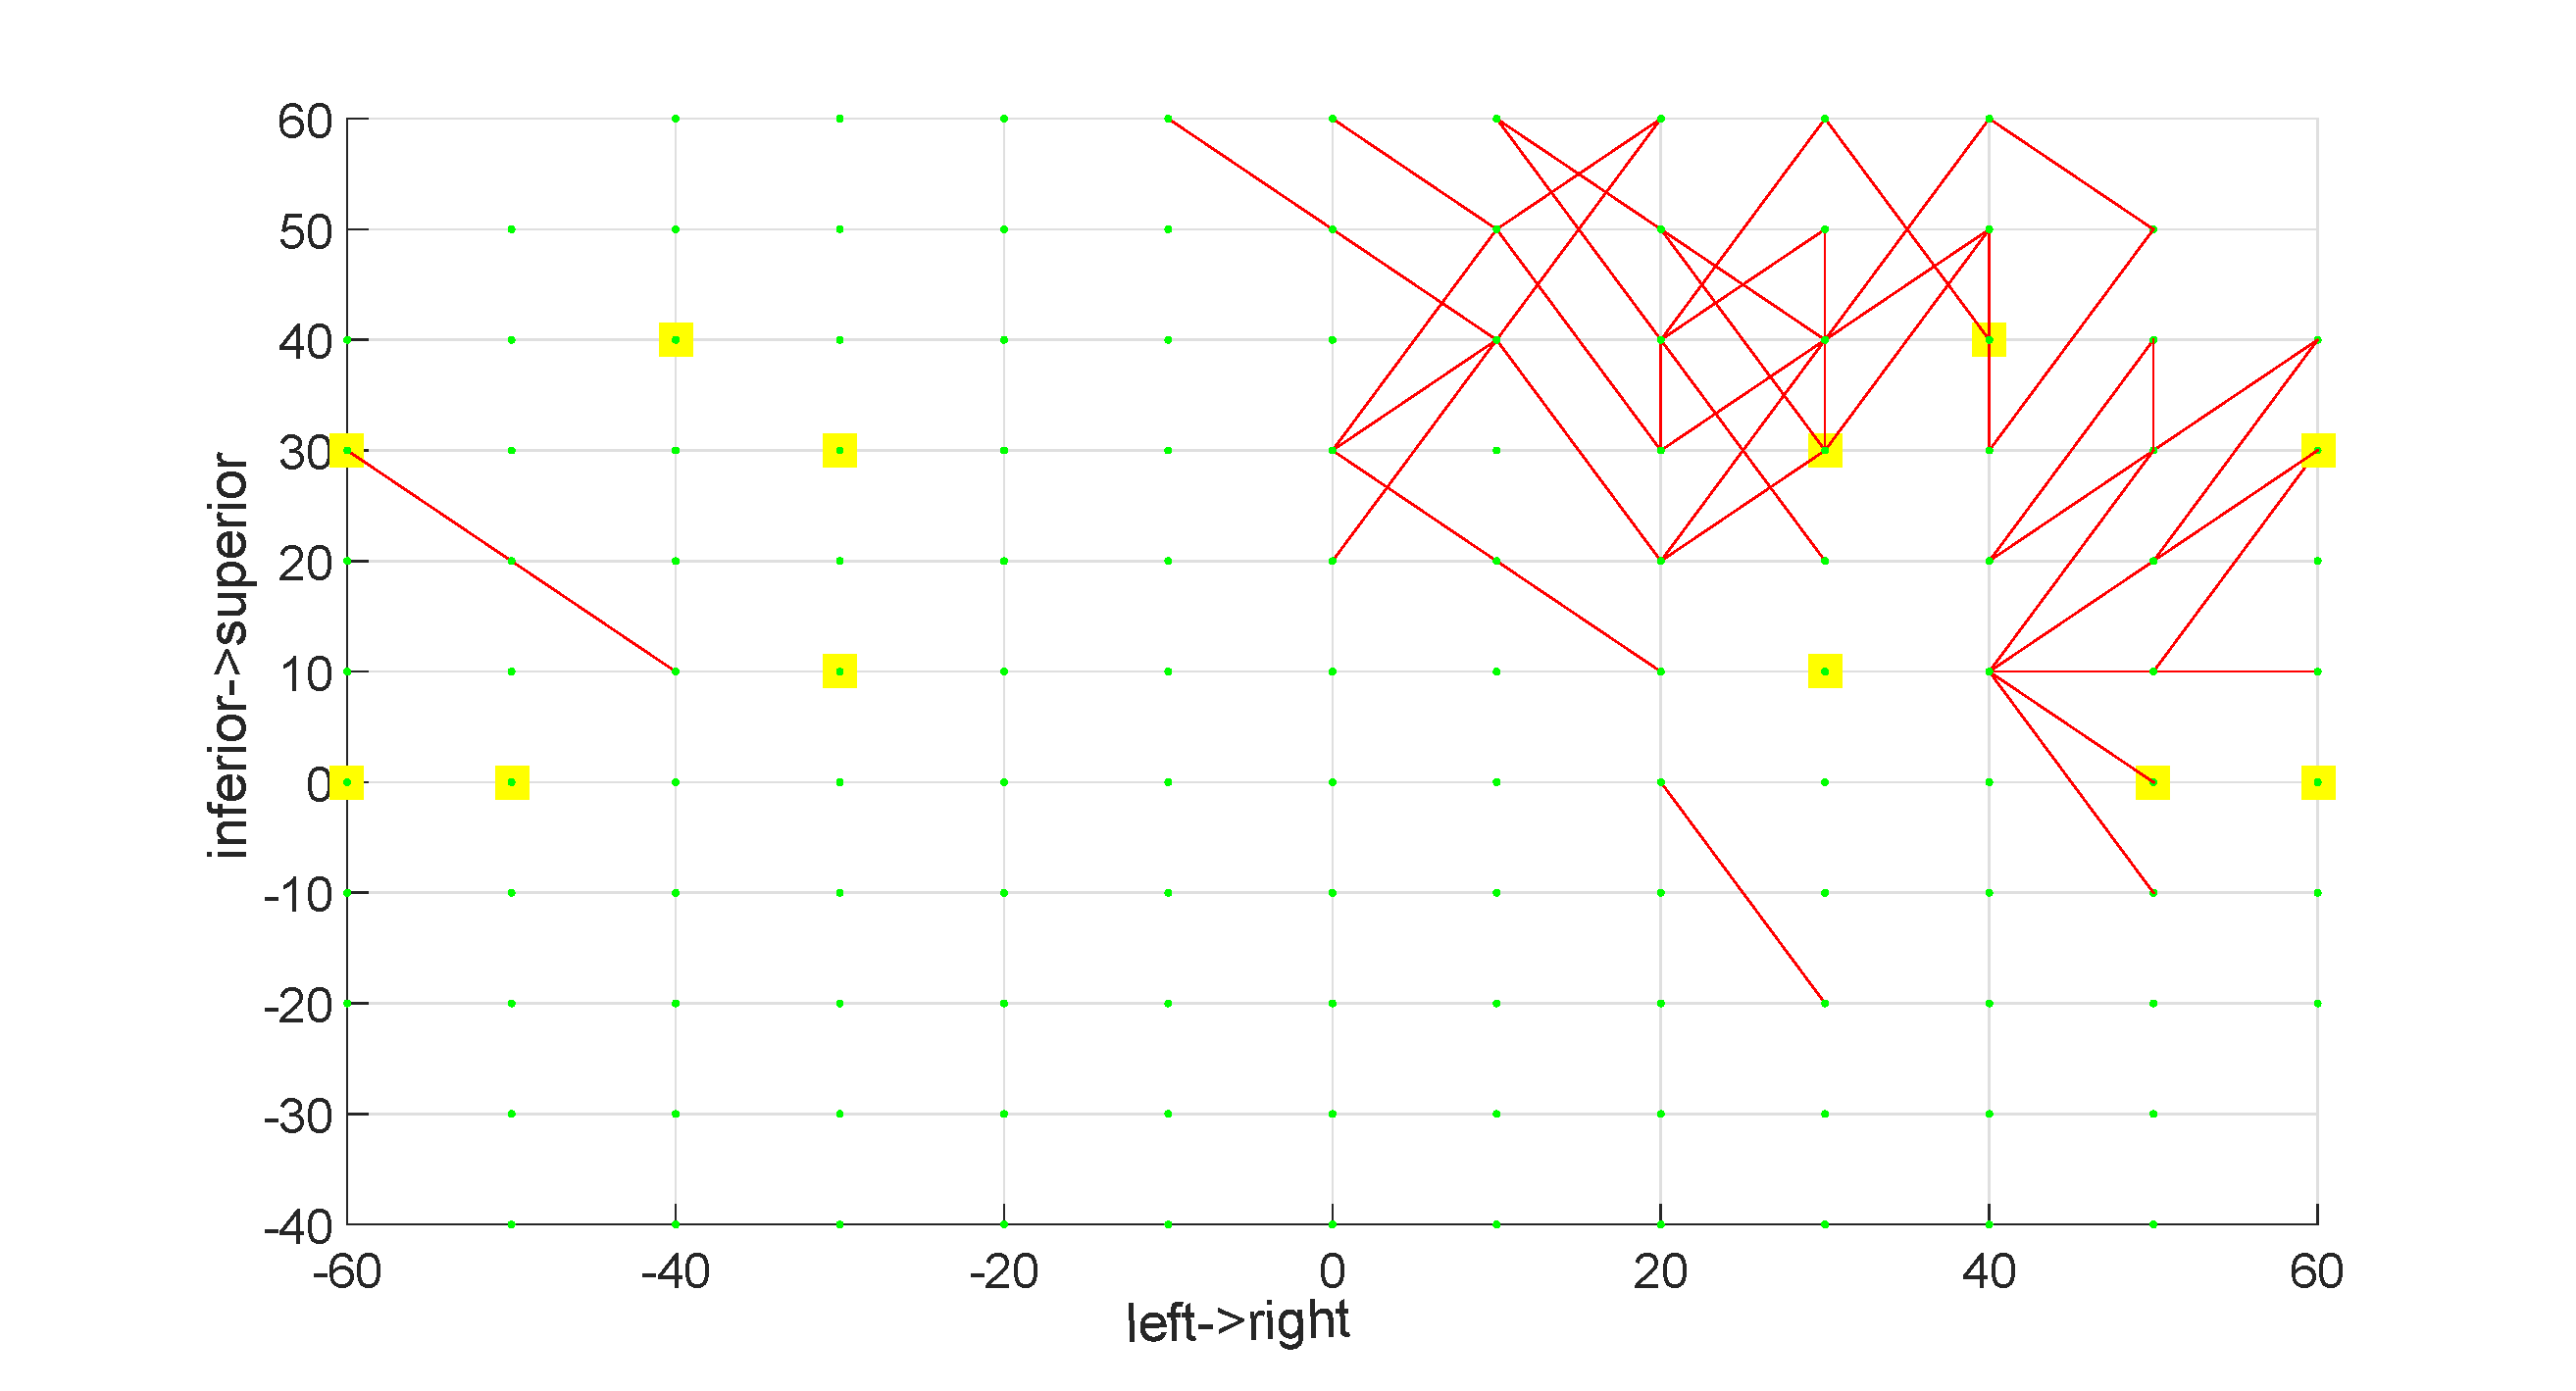
\includegraphics[scale=0.12]{fig/fmridti/ffxz.eps}}\\
	
	\subfloat[3D view]{\label{ex5}
		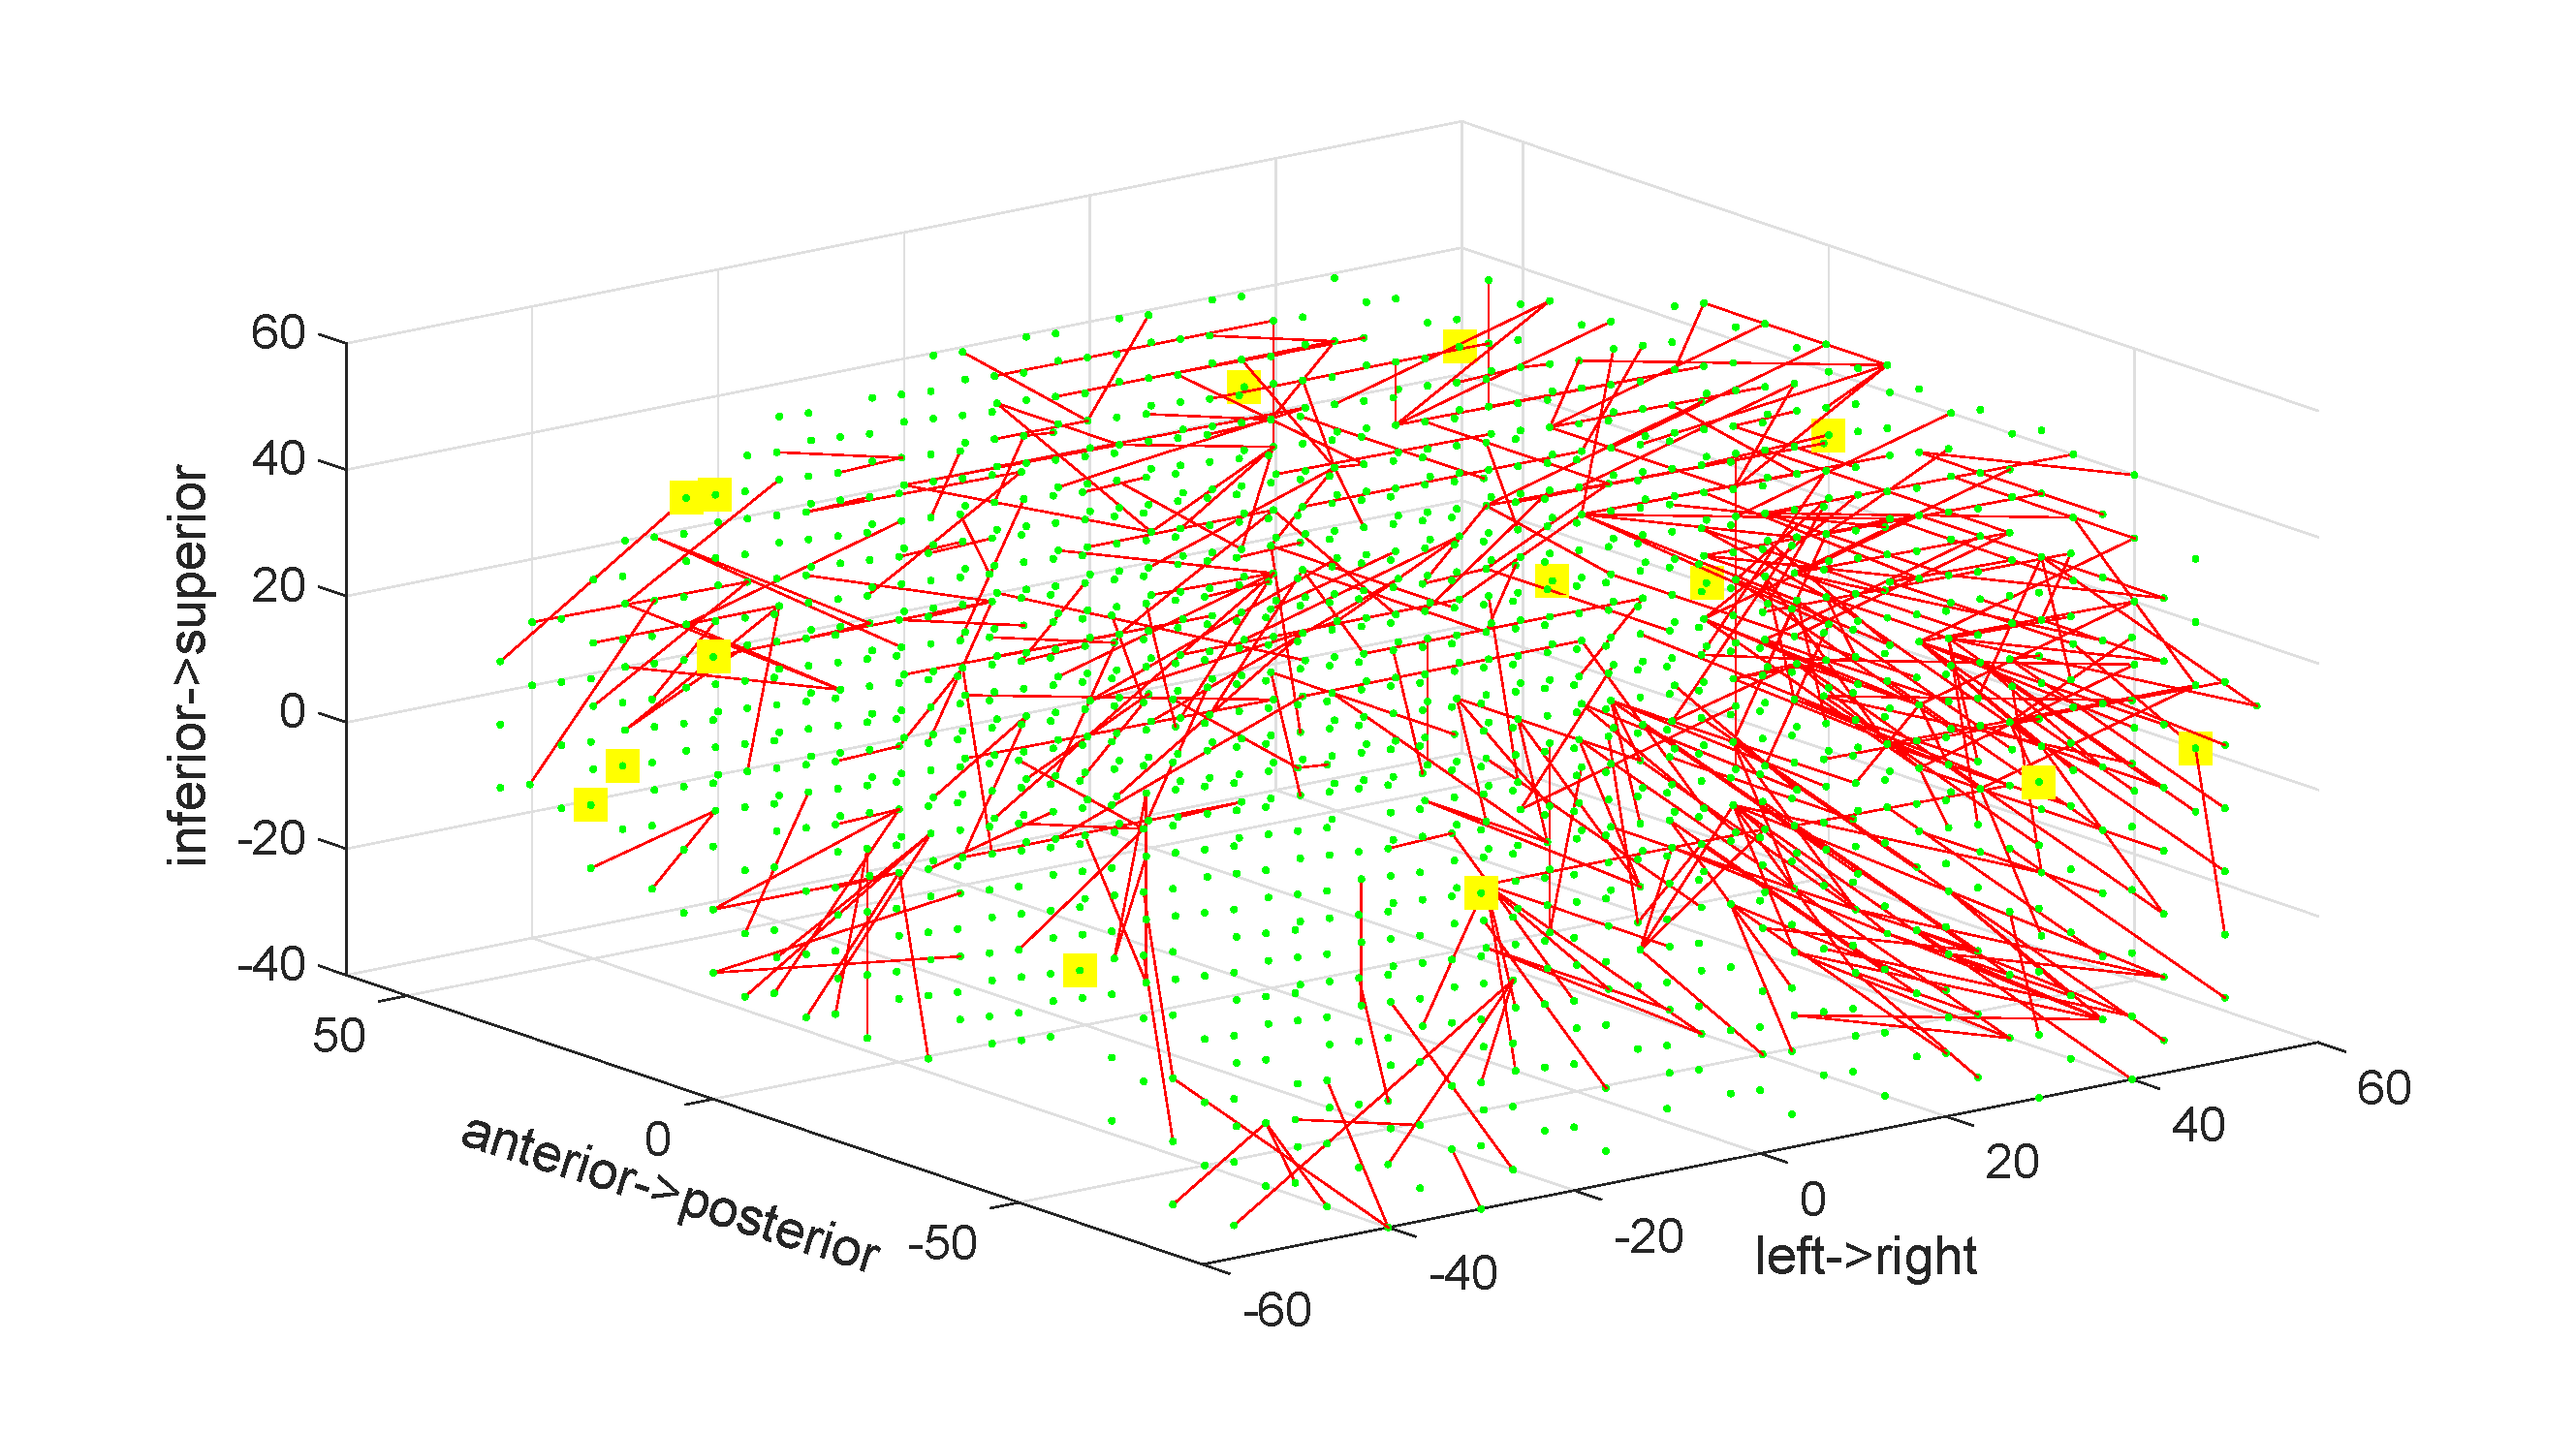
\includegraphics[scale=0.12]{fig/fmridti/nc3d.eps}}
	\subfloat[Horizontal view]{\label{ex51}
		\includegraphics[scale=0.12]{fig/fmridti/ncxy.eps}}
	\subfloat[Coronal view]{\label{ex6}
		\includegraphics[scale=0.12]{fig/fmridti/ncxz.eps}}
	\caption{The columns show the 3D, horizontal and coronal view of the strongest connection weights in the 3D SNNc at the end of the unsupervised learning. Each row corresponds to a different input orientation data. Every neuron of the SNN in the first row were simulated with orientation data ($\alpha=0$\textdegree, $\beta=0$\textdegree). This resulted in the majority of the strong connections being oriented in the direction ($alpha=0$\textdegree, $\beta=0$\textdegree). This shows the systematic bias towards orientation information in absence of any dynamic bias. The second row shows similar systematic bias towards the input orientation ($\alpha=45$\textdegree, $\beta=45$\textdegree). The third row is the baseline with no orientation influence where no systematic orientation information bias can be observed.}
	\label{fig:angle_effect}
\end{sidewaysfigure}
To analyse the behaviours of the oiSTDP learning algorithm, synthetically generated dynamic spatio-temporal data $D_{seq}$ and static orientation data $D_{stat}$ have been used. The input spike data $D_{seq}$ is of size $128 \times 14$, and was generated in a way that it mimics a random one second sample of a $128 Hz$ $14$ channel EEG device. The current experiment included $M=1485$ neurons with sparse recurrent connections. The neurons in the SNNc are spatially distributed to resemble the shape of the brain \citep{kasabov2014neucube}. The location of the input neurons in the SNNc are resolved as per the natural spatial ordering of EEG channels-AF3, F7, F3, FC5, T7, P7, O1, O2, P8, T8, FC6, F4 and F8. For connection generation, $r_{swc}=0.02$ (meaning connect neurons within $2\%$ of the maximum distance), and $W_{0}=0.05$, have been used. The spiking neurons are simulated using the parameters ($\eta_{thr}=4, v_{thr}=0.1, \kappa_-=\kappa_+=0.01$). 

\subsection{Effect of the Orientation Information on SNNc}
This segment demonstrates the systematic effect of orientation information in the SNNc map via the orientation influence $\psi$. The oiSTDP learning rule represents orientation information in conjunction with the spatio-temporal information in the connection strengths. The sample $D_{seq}$ was taken from a Poissons' distribution to keep minimal spike synchronicity in the data. This is done to minimise the influence of synchronicity to the maximum. As per \algorithmname \ref{alg:oiSTDP}, absence of synchronicity will mean that the spike data has minimal influence in the SNNc weight update. \figurename \ref{fig:angle_effect} shows the systematic effect of different input orientation information on the final 3D SNNc map. In first of three experiments, all the SNNc neurons were fed with input orientation data ($\alpha=0$\textdegree, $\beta=0$\textdegree), \emph{i.e.} parallel to the X axis and perpendicular to the Z axis. It is clearly visible from \figurenames \ref{ex00}, \ref{ex0} and \ref{ex1} that the strongest connections in the SNNc are formed in the direction of the orientation information provided. The second and third experiment use ($\alpha=45$\textdegree, $\beta=45$\textdegree), and no orientation information respectively. It is evident from \figurename \ref{fig:angle_effect} that in absence of the temporal information (synchronicity), the orientation information is reflected in the strongest connections of the SNNc, and, as such, in simple cases, they are visually discriminatory.

\subsection{Effect of the spike synchronicity on SNNc}
The aim of this experiment is to show the effect of spike synchronicity, \emph{i.e.} the effect of STDP learning (\equationname \ref{eq:stdp_online}) on the SNNc map for different spatio-temporal patterns. Per the STDP learning rule, greater synchronicity leads to stronger connections through LTP. To demonstrate the effect of the spatio-temporal synchronicity, two samples of the input spike data have been created. In the first sample, the spike sequences corresponding to the channels in the frontal lobe of the brain are kept the same (mimicking $100\%$ synchronicity) and in the second sample, $100\%$ spike synchronicity is kept at the occipital and parietal lobe. \figurename \ref{fig:activity_effect} shows the comparison between the two SNNc maps created by the oiSTDP learning algorithm when fed with these two samples. The `strongest connection' density is clearly more prominent in the frontal lobe in \figurename \ref{fig:effect_ex0} due to the greater input spike synchronicity in that region. Similar clusters (\figurename \ref{fig:effect_ex1}) at the parietal and occipital lobe can be seen with when the second sample is used. Through these analyses, it has been demonstrated how different temporal patterns and the spatial arrangement of such patterns can affect the visual map of SNNc through the oiSTDP learning.

\begin{figure}
\centering
	\subfloat[Synchronous input spike train at locations AF3, F7, F3, FC5, FC6, F4, F8 and AF4 (Horizontal view)]{\label{fig:effect_ex0}
		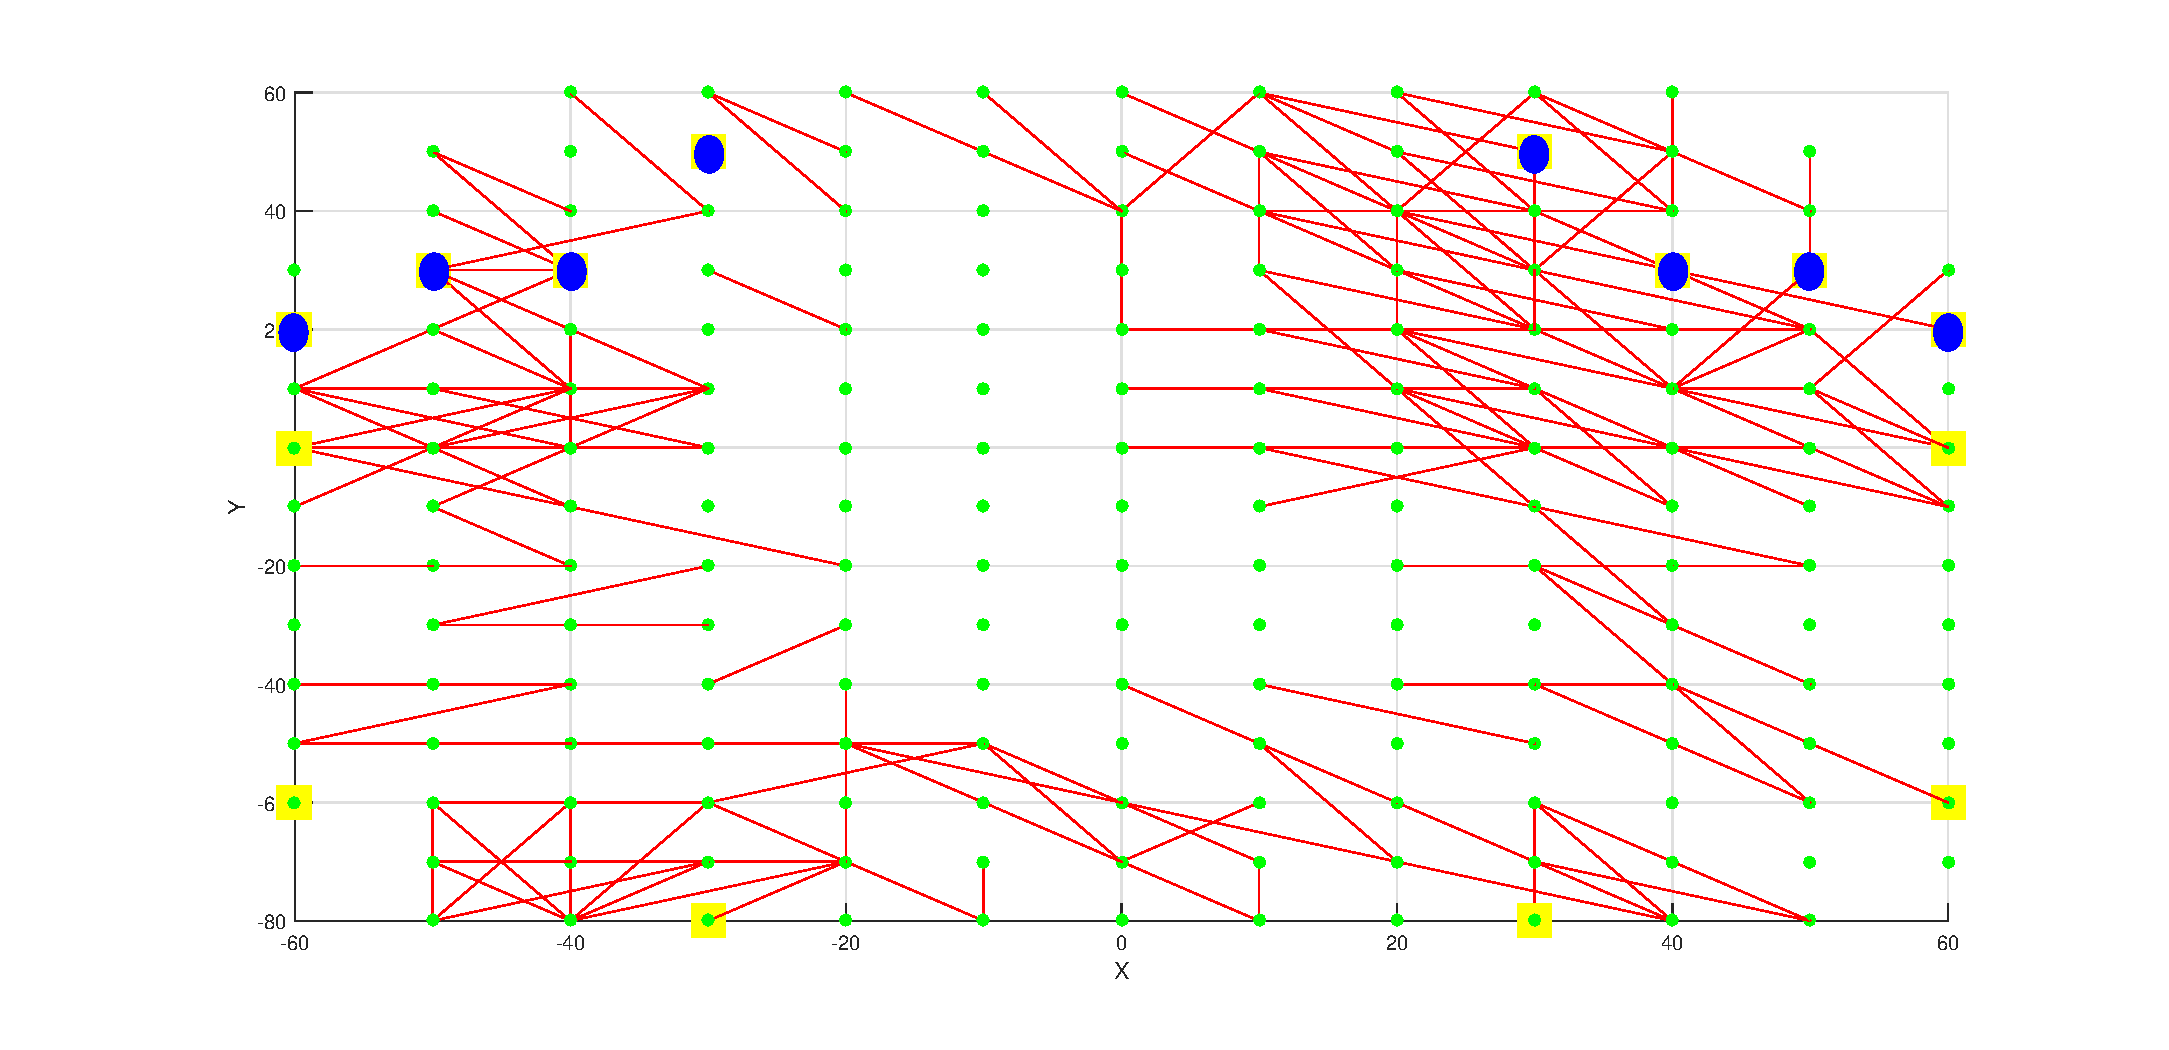
\includegraphics[width=0.5\textwidth]{fig/fmridti/activityeffectfrontxy.eps}}\hfill
	\subfloat[Synchronous input spike train at locations P7, O1, O2 and P8 (Horizontal view)]{\label{fig:effect_ex1}
		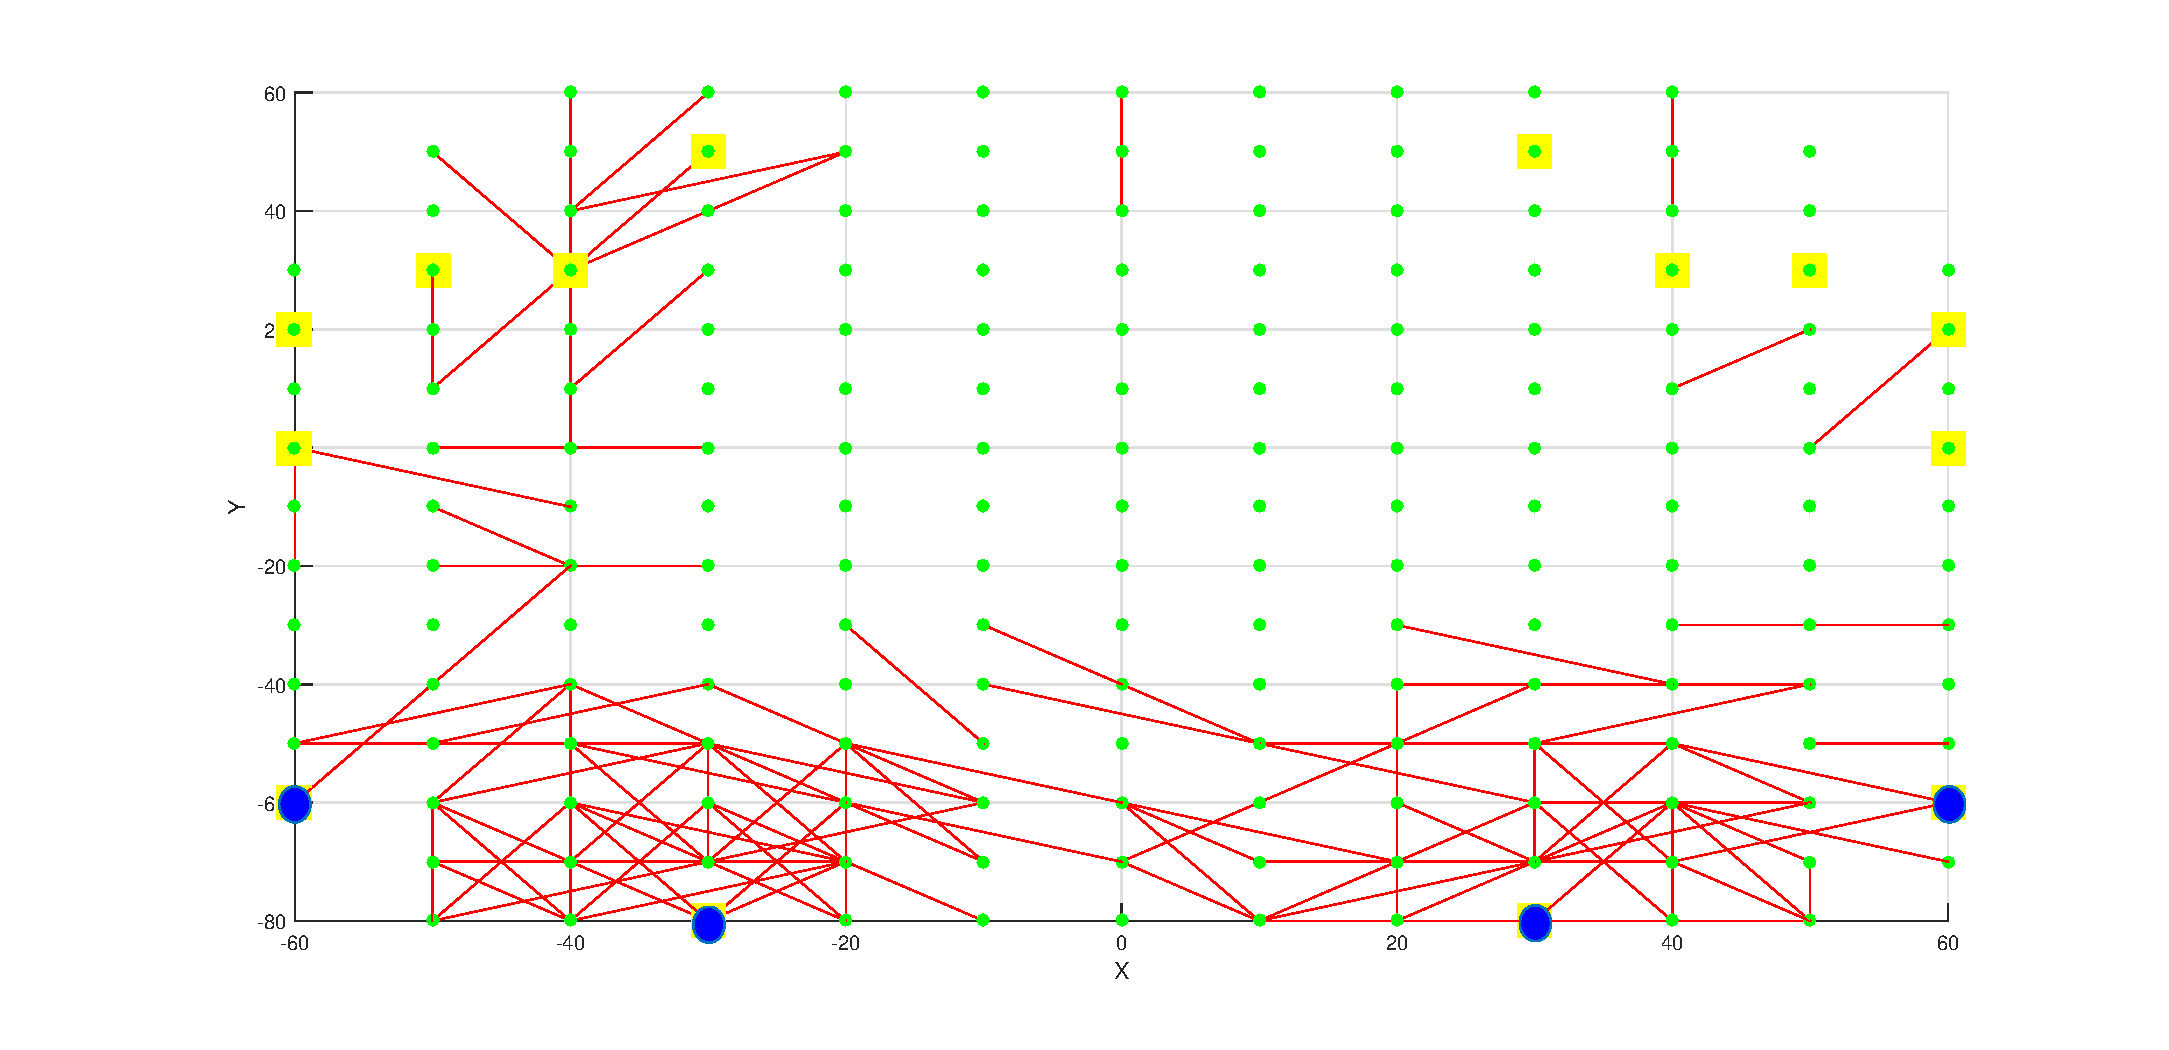
\includegraphics[width=0.5\textwidth]{fig/fmridti/activityeffectbackxy.eps}}
	\caption{Comparison of the effect of synchronous input spikes on the SNNc map generated by \algorithmname \ref{alg:oiSTDP}. The blue dots show the synchronous input channels.}
	
	\label{fig:activity_effect}
\end{figure}

\section{Personalised Predictive Modelling of Treatment Outcome using NeuCube with oiSTDP Learning}
\label{subsec:case-study}

This study was conducted as part of a large cross-sectional TRS study investigating Clozapine (CLZ) response in people with treatment resistant schizophrenia using EEG, MRI and genetic information. This study is a collaborative work with the school of pharmacy, University of Auckland. The University of Auckland conducted the participant recruitment, data collection and preprocessing. The current study's concentration and contribution lies in the data preprocessing, computational method development and data analysis. Strong efforts have been made to include all the relevant information in this study. However, for in-depth detail about the study, participants, data acquisitions and so on, the PhD thesis of \citet{mcnabb2017thesis} is a highly recommended read. This study was approved by the Health and Disability Ethics Committee and received locality approval from Auckland and Counties Manukau, District Health Boards of New Zealand. The ethical approval was obtained by the University of Auckland and a copy of the approval is attached in Appendix \ref{app:ethical_approval}.

\subsection{Schizophrenia and Antipsychotics}

The Global Burden of Disease Study, in 2013, estimated that $23$ million people, across the globe, were living with schizophrenia \citep{vos2015global}. Taking into account fewer than $0.01\%$ of the total population (though it was previously reported by \citet{mcgrath2008schizophrenia} the prevalence rates between $0.3\%$ and $0.7\%$), schizophrenia was found as a leading cause of years lived with disability and contributed to $3.7\%$ of the global burden of disease \citep{vos2015global}. The annual national expenditure of schizophrenia, in a systematic review, was estimated to range between USD $92$ billion and USD $102$ billion, with indirect costs accounting for $50\%$ to $85\%$ of the overall cost \citep{chong2016global}.

Schizophrenia most commonly emerges during adolescence or early adulthood \citep{spitzer1980diagnostic}. This disease is a leading cause of disability in individuals aged between $15$ and $44$ years \citep{rossler2005size}. Schizophrenia affects its targets through hallucination, reduced emotional expression and relapsing episodes of delusions, along with persistent cognitive dysfunction and several other disruptive symptoms that hinder an individual’s capacity to be an active and engaged member of society, thereby greatly diminishing their quality of life \citep{spitzer1980diagnostic}. Pharmacological treatment is one of the most successful tools for managing the symptoms affiliated with schizophrenia and has been shown to be effective in the majority of instances \citep{matheson2014much}. Nevertheless, despite best-practice, there are a small number of individuals who remain symptomatic. It has been estimated that as few as $5\%$ to as much as $60\%$ of the population inflicted with schizophrenia are resistant to first-line treatment \citep{elkis2007treatment, lehman2004practice, essock1996clozapine, juarez1995effects}. Contributing to some of the highest rates of hospitalisation and diminished functioning in mental health \citep{iasevoli2016treatment, lieberman2012comprehensive}, resistance to first-line antipsychotic intervention is estimated to cost USD $34$ billion per annum in healthcare expenditure within the US alone \citep{kennedy2014social}. Relieving patients of their most incapacitating symptoms, the atypical antipsychotic clozapine (CLZ) has been shown to be effective for treating between $30\%$ and $70\%$ of individuals who fail first-line treatment \citep{elkis2007treatment, essali2009clozapine, kane2016role}. The severe and potentially life-threatening side-effects linked to CLZ, however, restrict its use in the clinic. There are no current means for identifying those who will respond to treatment with CLZ, or alternatively, for identifying who will fail to respond to first-line therapy.

\subsection{Treatment Outcome in People with Schizophrenia}

Since the advent of chlorpromazine during the middle of the twentieth century, pharmacological interventions have been recognised as an integral component of treatment of people with schizophrenia. Nevertheless, treatment using first-line antipsychotics has been shown to be effective in only $60\%$ to $80\%$ of individuals. Fewer options for treatment exist for those who do not respond to first-line therapy, thereby leaving many patients without an effective means for managing their symptoms. Research suggests that CLZ can successfully treat treatment-resistant schizophrenia (TRS) \citep{meltzer2010role, kane1988clozapine}, resulting in significant enhancements towards quality of life, as well as positive long-term functional outcomes in some individuals \citep{essali2009clozapine}. However, CLZ also has the potential to cause serious, life-threatening side effects, such as agranulocytosis, myocarditis and cardiomyopathy, and has therefore, been restricted in its use, leading to delayed access for many individuals \citep{wheeler2008treatment}. Due to its noteworthy potential to cause improvement, psychiatrists are in need of reliable tools that can predict whether CLZ will be both an effective and a safe option for clients with schizophrenia.

Evidence suggests that schizophrenia is linked to disruptions to structural and functional connectivity \citep{yu2012brain, fitzsimmons2013review}. Work from previous research also suggests that functional connectivity may be different between individuals who respond to CLZ and those who are ultra-treatment-resistant (UTRS) \citep{creese1976dopamine, knott2000eeg}. \citep{rodriguez1996spect} found that lower perfusion in the thalamus, left basal ganglia and right prefrontal regions are poor responders to CLZ prior to treatment, and that individuals who have high metabolic activity in the dorsolateral prefrontal cortex were more likely to experience improvements in negative symptoms after administrating CLZ. Another study found improvements in the Positive and Negative Syndrome Scale (PANSS) correlated with pretreatment inter- and intra-hemispheric spectral power asymmetry, which was measured using electroencephalography (EEG) \citep{knott2000eeg}.

Pattern recognition algorithms can provide a novel and practical means to understand the differences between patients and healthy controls and predict individual patients' responses to treatment. Within psychiatric research, in particular, machine learning has gained considerable momentum as a useful tool for developing predictive models of treatment response. Incorporation of multiple imaging modalities into these algorithms could provide increased reliability, especially in disorders where clinical diagnosis does not necessarily guide treatment. \citet{patel2015machine} recently applied machine learning algorithms to predict treatment response in late-life depression using a combination of clinical and imaging data. Comparing several algorithms, they determined that alternating decision trees could most accurately predict treatment outcome in this cohort using a combination of structural and functional connectivity data \citep{patel2015machine}. \citet{khodayari2013machine} have used EEG data to predict the response to selective serotonin reuptake inhibitors in major depressive disorder and to CLZ in people with treatment-resistant schizophrenia \citep{khodayari2010pilot}. \citet{lin2008artificial} also employed machine learning algorithms to predict the response to CLZ, instead of using a combination of clinical and pharmacogenetic data as input. \citet{doehrmann2013predicting} employed machine learning techniques to predict treatment outcome in social anxiety disorder. Using task-based fMRI, they accounted for 40\% of the variance in treatment response \citep{doehrmann2013predicting}. The challenge now is to create an algorithm that can incorporate brain data from different modalities.

\subsection{Method}

\label{subsec:schizophrenia_method}

\subsubsection{Participants}

In accordance with the Diagnostic and Statistical Manual of Mental Disorders (DSM-IV), persons with a diagnosis of schizophrenia were recruited from mental health clinics within the Waitemata and Counties Manukau districts of Auckland, New Zealand. Participants were required to be: between the ages of 18 and 45; and clinically stable for at least six weeks prior to their inclusion in the study and also receiving atypical antipsychotics for the treatment of schizophrenia. Approximately twenty psychiatrically healthy control participants were also recruited as part of the research. The exclusion criteria involved current or previous diagnosis of any other axis I disorder, history of traumatic brain injury producing loss of consciousness of longer than three minutes, along with other significant physical disorders that were uncontrolled and may have affected brain structure, active substance dependence and contraindications for MRI. It is also noteworthy that participants were excluded from analysis if their functional image or supporting fieldmap image was overwhelmingly disrupted by motion. 

As per the history of treatment and current antipsychotic regimen, participants were assigned into one of three studies: “first-line responder” (FLR); “treatment resistant” (TRS); and “ultra-treatment resistant” (UTRS). The FLR group involved those responding well to first-line atypical antipsychotic mono-therapy. The TRS group consisted of participants who failed at least two previous six-to-eight-week trials of atypical antipsychotics and were now receiving CLZ. Lastly, those who failed at least two previous six-to-eight-week trials of atypical antipsychotics and had also failed a trial of CLZ monotherapy were enrolled in the UTRS group. Participants in the UTRS group all received a mixture of two antipsychotic drugs; $79\%$ received CLZ as part of an augmented treatment method.

The demographics of the participants were compared across cohorts using IBM SPSS Statistics Version 24. The Student’s t-test was used to analyse the variables that satisfied assumptions of homoscedasticity (Brown-Forsythe test for equality of variances) and normality (Shapiro-Wilk test for normality). Variables that violated assumptions of homoscedasticity and/or normality were analysed using the Mann-Whitney U tests or Z-score.


\subsubsection{Data Acquisition}

The Siemens Mangetom Skyra 3T scanner at the Centre for Advanced MRI (University of Auckland, New Zealand) was used to acquire the diffusion and resting-state (rs) functional magnetic resonance images. Magnetisation prepared 180-degrees radio-frequency pulses and rapid gradient-echo (MPRAGE) sequence were used to obtain Structural T1-weighted images. These were the acquisition parameters: Repetition time (TR) $1900$ ms; echo time (TE) $2.39$ ms; inversion time (TI) $900$ ms; flip angle $9$\textdegree; repetition $1$; acceleration (GRAPPA) factor of $2$; field of view (FOV) $230$ mm; matrix $256 \times 256$; voxel size $0.9 \times 0.9 \times 0.8$ mm. 

Diffusion-weighted (DWI) images were obtained through an echo planar imaging (EPI) sequence with the following parameters: TR $8900$ ms, TE $95$ ms, FOV $240$ mm, $122 \times 122$ matrix, $2.0$ mm slice thickness, isotropic voxel size $2.0 \times 2.0 \times 2.0$ mm. An acceleration factor of $2$ was used. $67$ slices were acquired parallel to the anterior commissure-posterior commissure ($A >> P$) direction with diffusion-weighting factor $b=1000$ s/mm2 in $64$ gradient directions. There were a further $8$ scans without diffusion weighting ($b=0$ s/mm2) which were also acquired. 

Gradient distortion (fieldmap) images for diffusion data were acquired using a gradient echo pulse sequence with the following parameters: TR $655$ ms; TE1 $4.92$ ms; TE2 $7.38$ ms; voxel size $3.8 x 3.8 x 2.0$ mm; phase encode direction $R >> L$; FOV $240$ mm. 

Rs functional images were acquired using EPI with the following parameters: TR $3000$ ms, TE $30$ ms; echo spacing $0.65$ ms ($0.62$ ms for last $4$ participants, following software upgrade); phase-encode direction $A >> P$; slices $54$; volumes $160$; FOV $192$ mm; acceleration factor of $2$; matrix $64 \times 64$; voxel size $3.0 \times 3.0 \times 3.0$ mm. Participants were requested to lie immobile with eyes open and to focus their attention on a fixation cross that was presented on a screen in front of the scanner. Participants were given the instruction to keep a blank state of mind by not thinking of anything in particular.

Gradient distortion images for functional data were acquired using a gradient echo pulse sequence with the following parameters: TR $655$ ms; TE1 $4.92$ ms; TE2 $7.38$ ms; voxel size $3.4 \times 3.4 \times 2.4$ mm; phase-encode direction $A >> P$; FOV $220$ mm. 

\subsubsection{fMRI Image Preprocessing}
fMRI image preprocessing was performed using FSL version $5.0.7$ \citep{smith2004advances}. Brain tissue was extracted from raw magnitude files using FSL’s BET \citep{smith2002fast}, after which brain-extracted images were eroded to ensure that no voxels containing non-brain tissue remained. Fieldmaps were then created using the fsl\_prepare\_fieldmap function. Functional image registration to high resolution structural and MNI152 standard space was performed using FMRIB's Expert Analysis Tool (FEAT). Preprocessing parameters in FEAT were as follows: motion correction = MCFLIRT; b0 unwarping = on; echo spacing = $0.325$ ($0.31$ for last $5$ participants); TE = $30$; spatial smoothing = $5$mm; global intensity normalisation = on; temporal filtering = off; MELODIC = off; registration to structural image = boundary-based registration; registration to MNI152\_2mm = non-linear; warp resolution = $10$ mm. 

ICA-based Automatic Removal Of Motion Artefacts (ICA-AROMA) \citep{pruim2015ica} was used to remove motion artefacts from the fMRI data utilising FSL’s FEAT output as input. White matter and cerebro-spinal fluid (CSF) maps were segmented from high resolution structural images using FSL’s FAST \citep{zhang2001segmentation} and warped to functional space using linear registration to FEAT output (FSL’s FLIRT \citep{jenkinson2001global}). Nuisance time-series were generated from ICA-AROMA output (denoised functional data) using CSF and white matter maps as input. A general linear model (GLM) of residual activity was then generated from the denoised functional data and nuisance time-series using FSL’s GLM. A temporal mean file of denoised functional data was created, to which high-pass temporal filtering (sigma=$16.7$) was applied in addition to removal of residual activity attributed to CSF and white matter. Filtered, de-noised functional data was then warped to MNI standard space for use in further analysis.

\subsubsection{DTI Image Preprocessing}

DTI image preprocessing was performed using FSL version $5.0.7$ \citep{smith2004advances}. Structural images were reoriented to a standard template and brain tissue was extracted from raw image files using FSL’s brain extraction tool (BET) \citep{smith2002fast}. If automatic brain extraction failed to eliminate all non-brain tissue, the excess was removed manually. Magnitude images were subjected to the same process, after which brain-extracted images were eroded to ensure that no voxels containing non-brain tissue remained. Fieldmaps were then created using the fsl\_prepare\_fieldmap function. The gradient-free image was used to create a binary mask with BET. Gradient distortions were corrected using FSL’s fugue function and output registered to gradient-free images using the linear registration function (FLIRT) \citep{jenkinson2001global}. Data were then corrected for head movement and eddy current distortions using FSL’s eddy tool \citep{andersson2016integrated}. Slices with average intensity at least four standard deviations lower than the expected intensity were interpolated with predictions made by the Gaussian Process \citep{andersson2016incorporating}. DTIfit was used to independently fit diffusion tensors to each voxel, limited to brain space using the binary brain mask. Crossing fibres were modelled using Bayesian Estimation of Diffusion Parameters Obtained using Sampling Techniques (BEDPOSTX) \citep{behrens2003characterization}. BEDPOSTX estimates of primary fibre orientations (dyads1) were then warped to a standard MNI template for use in the initial NeuCube construction.

The second stage of data processing focused on selecting a set of voxels from the fMRI and DTI to be used to build the multi-modal NeuCube model. As discussed in Section \ref{sec: SNNc}, since a major component of this model captures temporal variations in data and the noise reduction capabilities of SNN architectures through encoding \citep{kasabov2016evolving}, it was hypothesised that the discriminatory information is hidden in the voxels with significant variability in the activity over time. A set of voxels with an absolute mean standard deviation of greater than $105$ were selected for the experiments. \figurename \ref{fig:vox_sel} shows the 3D atlas locations of the selected voxels in the MNI coordinate system. The selected voxels are found to be predominantly ($>67\%$) located in the cerebellum area of the brain. The second and third column of the ROI frequency table (see \tablename \ref{tab:vox_freq}) also lists to the number and the percentage of voxels belonging to the different ROIs.  

In this study, the aim was to build a model for discriminating CLZ mono-therapy respondent and non-respondent individuals from multi-modal fMRI and DTI brain data. For this investigation, a subset of data was collected from the TRS study with the intention of classifying subjects into groups with either TRS or UTRS using resting-state fMRI and DTI data. A total of $30$ subjects were chosen for the study. Sixteen subjects belonged to the TRS group and fourteen to the UTRS group. 

\subsubsection{Experimental Results}

         

\begin{table}
	\centering
	\caption{Frequency table of ROI's of the selected voxels.}
	\label{tab:vox_freq}
	\begin{tabular}{@{}ccc@{}}
		\toprule\toprule
		\textbf{ROI} & \textbf{$\#$ voxel} & \textbf{$\%$}\\ \midrule
		Frontal Lobe  &    $177$  &    $7.64$ \\ 
		Insula    &   $16$  &   $0.69$ \\ 
		Temporal Lobe   &   $138$  &    $5.95$ \\ 
		Cerebellum  &   $1557$  &   $67.17$ \\ 
		Occipital Lobe   &    $25$  &    $1.08$ \\ 
		Parietal Lobe    &  $134$  &    $5.78$ \\ 
		Thalamus   &   $187$  &    $8.07$ \\ 
		Caudate   &    $84$   &   $3.62$ \\
		\bottomrule\bottomrule
	\end{tabular}%
\end{table}           

\begin{figure}
	\centering
	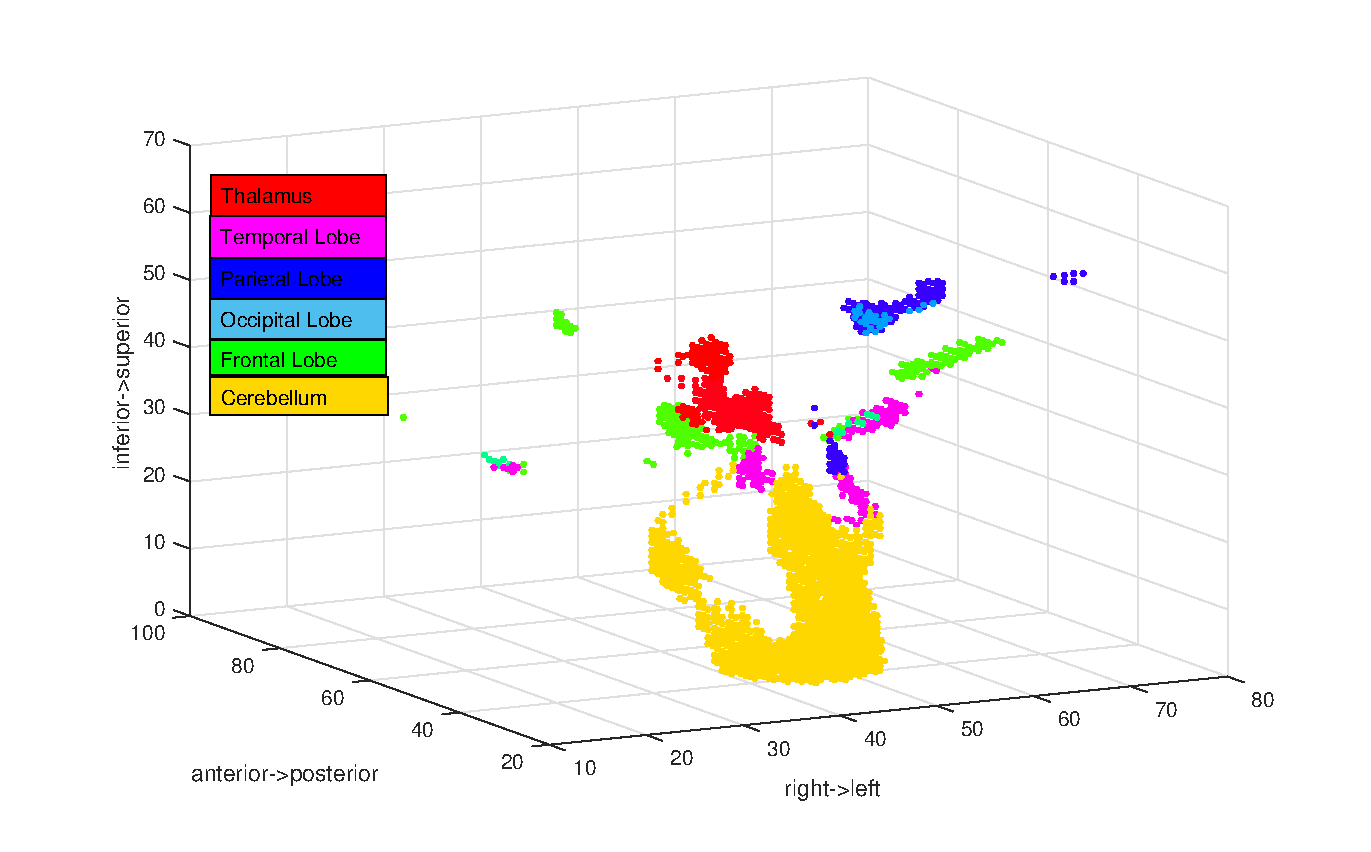
\includegraphics[width=\linewidth]{fig/fmridti//selectedvoxelsroi.eps}
	\caption{Voxel selection using absolute mean standard deviation.}
	\label{fig:vox_sel}
\end{figure}
The final preprocessed dataset consists of dynamic fMRI trials $\mathbf{D_{seq}} \in \mathbb{R}^{30\times 2318 \times 80}$ and static DTI orientation vector data $\mathbf{D_{stat}} \in \mathbb{R}^{30\times 2318 \times 3}$ of $30$ subjects and $2318$ voxels. Each fMRI voxel is sampled over $80$ time points within a trial. The voxels of the DTI orientation data are represented by 3D vectors signifying the primary orientation of the fibre tract at the voxel location.     

The NeuCube personalised architecture consists of three modules as described in Section \ref{sec: SNNc}. The first step of the process was to compress or encode the dynamic fMRI data from continuous real space to binary spike space. For the encoding step, the BSA \citep{schrauwen2003bsa} algorithm was chosen due to its ability to represent brain data as important spike event and has shown promising results in \citep{sengupta2017spike,nuntalid2011eeg}. For the second step, subject-specific SNNc's were initialised with $Q=1000$ spiking neurons, $N=2318$ input neurons and synapses were initialised using the SWC algorithm within the radial neighbourhood of $r_{swc}=0.05$ and $w_{ij}=0.05$. The spiking neurons were set with the hyperparameters $\{v_{rest}=0, v_{thr}=0.1, \eta_{thr}=8\}$. These along with other hyperparameters were chosen by a grid based hyperparameter search strategy. The encoded fMRI data and the DTI orientation vector data for each subject were then passed through the initialised SNNc, generating $O_{seq}$ for each subject using \algorithmname \ref{alg:oiSTDP}. In the final step, a lazy K-NN binary classification model using $50\%$ of the randomly chosen subjects was learned. It is to be noted that a custom distance function as part of the K-NN algorithm for learning binary spike data was used. A custom spike asynchronicity-based distance function as described in Section \ref{parag:knn_custom} and in \citep{sengupta2017spike} has been utilised. The K-NN learning algorithm can of course be replaced by any supervised learning module that can learn from discrete or binary input data.           

Due to the multi-modular and rather flexible nature of the NeuCube architecture, selecting baselines for comparison is a challenging task. In this work, the NeuCube architecture was used as a combination of temporal feature compressor, spatial expander and classifier. The compressor and the SNNc module together are used as a spatio-temporal feature extraction module. The supervised readout layer then learns a model from the transformed feature transformed data. Hence it is appropriate to compare the BSA+oiSTDP feature extraction module against other feature extraction methods in continuous data domain. The following feature extraction algorithms have been compared:
\begin{enumerate}
	\item Sparse autoencoder \citep{ng2011sparse}: Autoencoders are shallow single hidden layer neural networks that can perform identity mapping of the input. The hidden layer of the autoencoder learns non linear lower dimensional data representations. The sparse autoencoders are an extension of regular autoencoders that impose sparsity regularisation constraints on the loss function. In these present experiments, the fMRI data was used to learn a sparse autoencoder (with $1000$ relu units in the hidden layer and L1 regularisation constraint of $10^{-5}$) that encodes the data into $1000$ dimensional feature space using the python keras API \citep{chollet2015keras}.   
	\item Principal component analysis (PCA): PCA is a standard orthogonal linear feature transformation technique that transforms features into principal components. Using the scikit-learn API, $1000$ principal components were fitted and transformed on the fMRI data.
	\item Independent component analysis (ICA): ICA is another statistical feature transformation technique used to decompose feature space to statistically independent component space by maximising statistical independence of the estimated components. Once again, scikit-learn \citep{scikit-learn} API's FastICA algorithm was used to fit and transform the fMRI data to $1000$ independent components.  
	\item Restricted Boltzman's machine (RBM) \citep{hinton2006reducing}: RBM is an unsupervised nonlinear feature learner based on a probabilistic model that has gained much popularity in the deep neural network domain. The scikit-learn API \citep{scikit-learn} was used to learn a Bernoulli RBM network, with $1000$ components using stochastic Maximum likelihood \citep{tieleman2008training} learning. 
\end{enumerate}

\begin{table}
	\centering
	\caption{Comparison of the pattern recognition methods on the binary classification task.}
	\label{tab:class}
	\resizebox{\textwidth}{!}{%
		\begin{tabular}{@{}lll>{\centering\arraybackslash}m{2cm}>{\centering\arraybackslash}m{2cm}cc@{}}
			\toprule
			\toprule
			\multirow{2}{*}{\textbf{Method}} & \multirow{2}{*}{\textbf{Framework}\footnotemark[1]} & \multirow{2}{*}{\textbf{Data}} & \multicolumn{2}{c}{\textbf{Relation learning capabilities}} & \multicolumn{2}{c}{\textbf{Performance\footnotemark[2]}} \\ \cmidrule(l){4-5} \cmidrule(l){6-7}
			&  &  & Temporal &  Multi-modal & Accuracy ($\%$) & Cohen's $\kappa$ \\ \midrule
			\textbf{BSA+oiSTDP+K-NN(C)} & TFC+SE+C & fMRI+DTI & \cmark & \cmark & $\mathbf{72.3\pm 12.3}$ & $\mathbf{0.44\pm0.25}$ \\ 
			BSA+STDP+K-NN(C) & TFC+SE+C & fMRI & \cmark & \xmark & $69.4\pm 13.9$ & $0.38\pm 0.28$ \\ 
			BSA+K-NN(C) & TFC+C & fMRI & \xmark & \xmark & $64.2\pm 12.4$ & $0.22\pm 0.26$ \\
			Sparse Autoencoder+K-NN(E) & NTFC+C & fMRI & \xmark & \xmark &  $56.1\pm 7.2 $ & $0.01\pm 0.11$ \\
			PCA+K-NN(E) & NTFC+C & fMRI & \xmark & \xmark & $56.1\pm 11.3$ & $0.13\pm 0.18$ \\
			ICA+K-NN(E) & NTFC+C & fMRI & \xmark & \xmark & $62.8\pm 12.3$ & $0.26\pm 0.23$ \\
			RBM+K-NN(E) & NTFC+C & fMRI & \xmark & \xmark & $36.2\pm 4.9$ & $-0.23\pm 0.11$ \\
			LSTM  & C & fMRI & \cmark & \xmark & $45.7\pm 9.6$ & $-0.15\pm 0.14$ \\
			GRU & C & fMRI & \cmark & \xmark & $45.2\pm 7.5$ & $-0.018\pm 0.13$ \\ \bottomrule\bottomrule
		\end{tabular}%
	}
\end{table}

\footnotetext[1]{TFC=Temporal feature compressor, NTFC=No-temporal feature compressor, SE=Spatial expander, C=classifier}
\footnotetext[2]{The performance metrics are computed as $mean\pm standard\ deviation$ of $10$ independent train/test runs of the classification module}


\tablename \ref{tab:class} presents the experimental results. The rows of the table compares the methods for the classification task. (C) and (E) in the method names correspond to the custom and euclidean distance function used as part of K-NN respectively. The framework column specifies the role of each component in the method names. For example, the proposed BSA+oiSTDP+K-NN is a combination of temporal feature compressor (TFC), spatial expander (SE) and classifier (C). The Performance of the binary classification task is measured by overall accuracy and Cohen's $\kappa$ statistic. The first $3$ rows of the table compare the different NeuCube architectures. The BSA+oiSTDP+K-NN is the proposed architecture for fMRI and DTI integrated learning. The next two methods systematically removes (1) orientation influence from SNNc learning (STDP) and (2) the SNNc module to show the effect of inclusion of these artefacts on the performance. The best performance across the different methods is achieved by the proposed BSA+oiSTDP+K-NN architecture with overall accuracy of $72.4\pm 12.3\%$ and Cohen's kappa of $0.44\pm 0.25$. The classification accuracy increases by $\approx 8\%$ and doubles the mean Cohen's $\kappa$ statistic when oiSTDP-based SNNc learning is performed in the middle using fMRI and DTI data. Rows $4$ to $7$ are the non temporal feature extraction baselines described earlier. Due to the non temporal nature of the baseline feature compressors, the fMRI data for each subject is input to these feature extractors as a single vector (created by concatenating the temporal dimension) leading to a massive feature vector space. K-NN ($K=1$) classifier was used for the classification task to keep the comparisons as fair as possible. The disadvantage of the large feature space is quite imperative as it leads to potential over fitting of the data. The DTI data was not added to the already large feature space to avoid further over fitting. As the SNNc of NeuCube is a spiking recurrent neural network framework with temporal or sequential learning capabilities, the binary classification task with other single hidden layer recurrent neural network framework, such as long short term memory (LSTM) \citep{hochreiter1997lstm} and gated recurrent units (GRU) \citep{cho2014learning} was also brought to light. Both LSTM and GRU networks were designed as shallow single hidden layered neural networks having $50$ LSTM and GRU units. These networks were implemented in keras API \citep{chollet2015keras} and learned by optimising the binary crossentropy loss function using the adaptive momentum optimiser. The results for the baselines show that K-NN performs best on ICA-based feature representation. PCA and sparse autoencoders are similar in accuracy, but PCA achieves a stronger $\kappa$ statistic. On the other hand, the baseline recurrent neural networks fail to learn the task, leading to poor performance statistics.              
\begin{sidewaysfigure}
	\centering
	\subfloat[Horizontal view]{\label{fig:toptrs}
		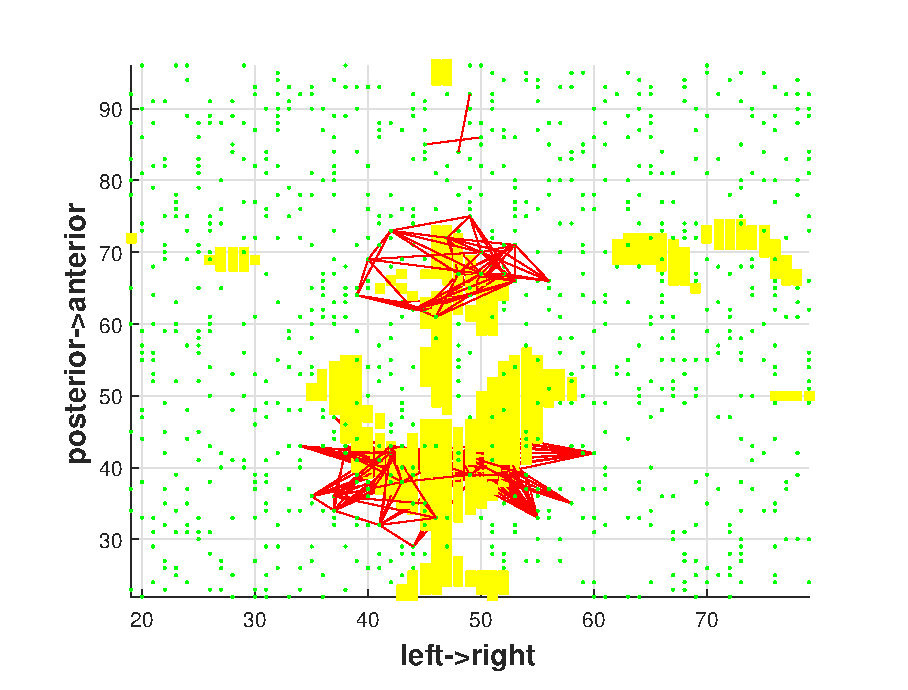
\includegraphics[width=0.32\linewidth]{fig/fmridti/meanweightTRSth065xy.eps}}
	\subfloat[Coronal view]{\label{fig:backtrs}
		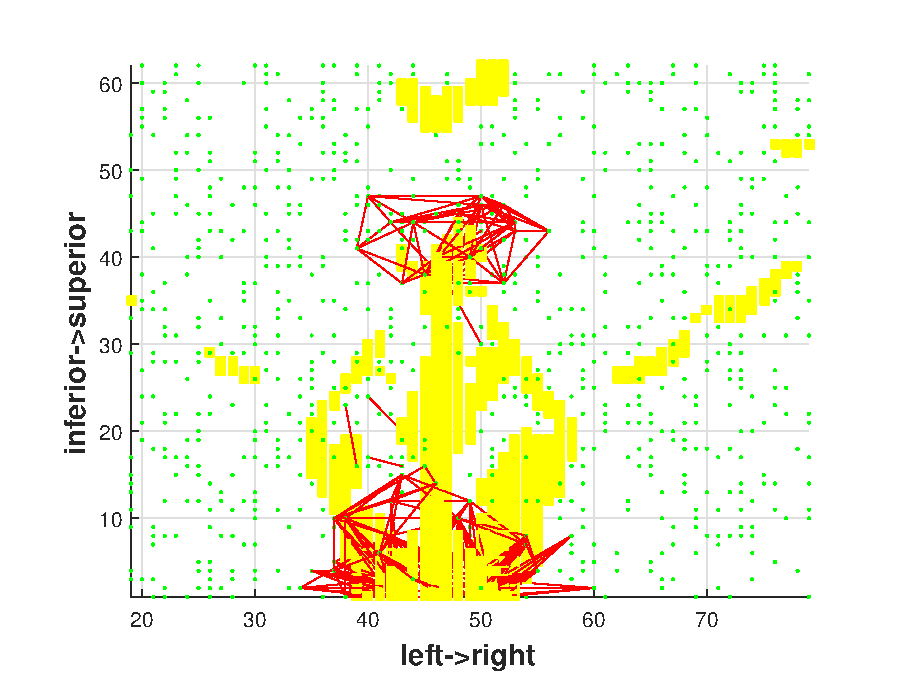
\includegraphics[width=0.32\linewidth]{fig/fmridti/meanweightTRSth065xz.eps}}
	\subfloat[Sagittal view]{\label{fig:sidetrs}
		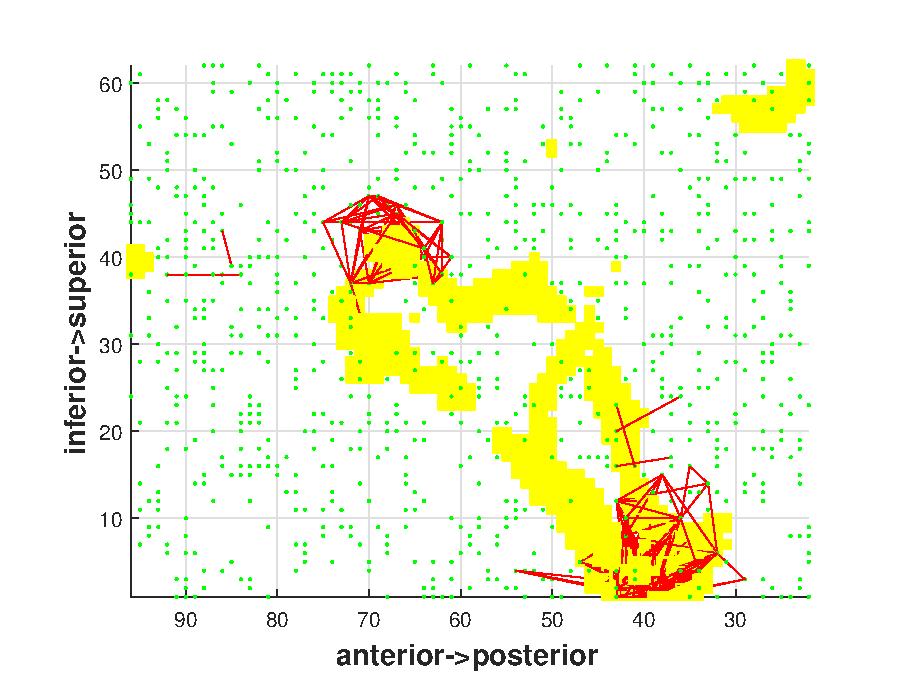
\includegraphics[width=0.32\linewidth]{fig/fmridti/meanweightTRSth065yz.eps}}\\	
	\subfloat[Horizontal view]{\label{fig:toputrs}
		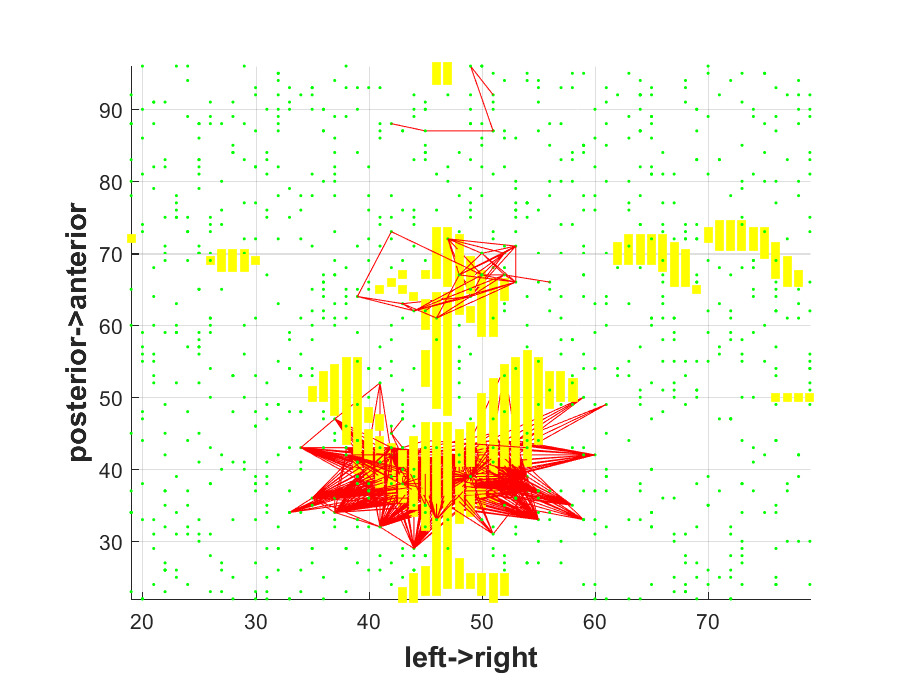
\includegraphics[width=0.32\linewidth]{fig/fmridti/meanweightUTRSth065xy.eps}}
	\subfloat[Coronal view]{\label{fig:backutrs}
		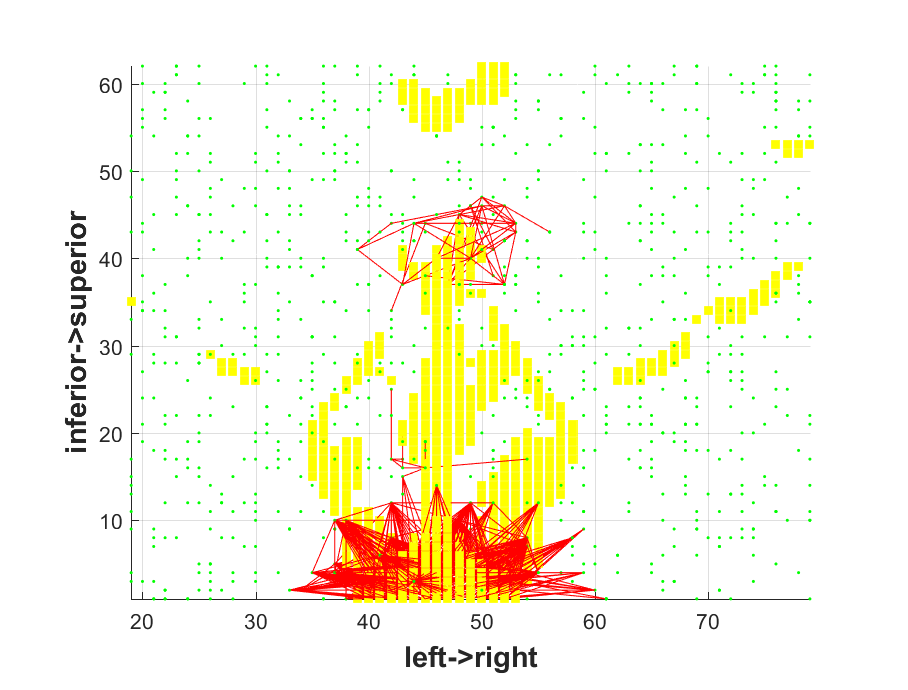
\includegraphics[width=0.32\linewidth]{fig/fmridti/meanweightUTRSth065xz.eps}}
	\subfloat[Sagittal view]{\label{fig:sideutrs}
		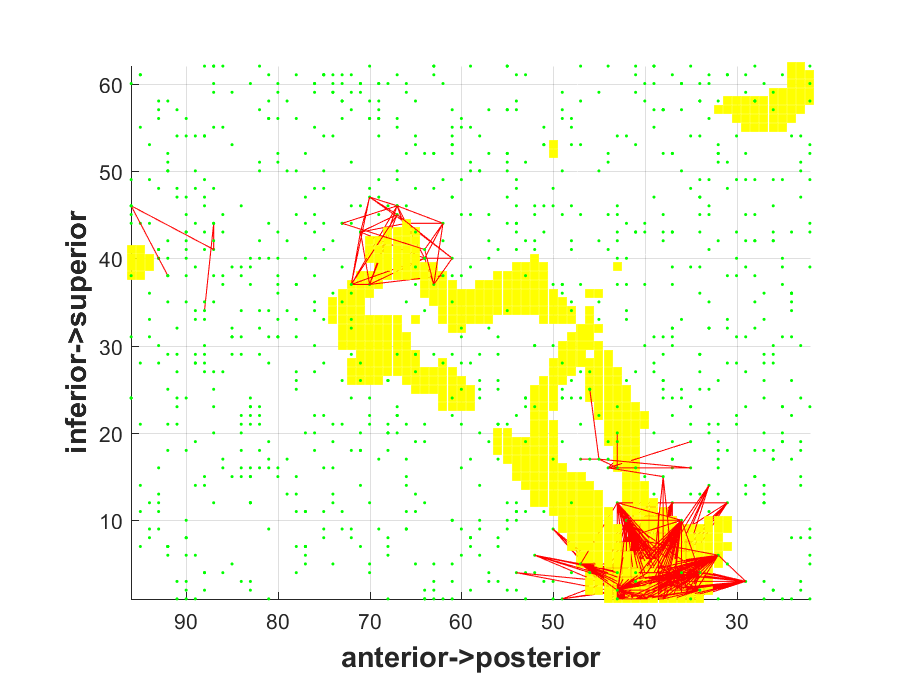
\includegraphics[width=0.32\linewidth]{fig/fmridti/meanweightUTRSth065yz.eps}}\\
	\caption{A visual comparison of the strongest connections (mean weight across subjects within a group) formed in the SNNc of the TRS and the UTRS group. The top row shows the connections in the TRS group and the bottom row corresponds to the UTRS group. The yellow coloured cluster represents the input neurons and the green neurons are the computational spiking neurons.}
	\label{fig:clz_TRS_UTRS}
\end{sidewaysfigure}

Furthermore, connection weights have been individually scrutinised for the TRS and the UTRS group, generated by the oiSTDP learning algorithm. \figurename \ref{fig:clz_TRS_UTRS} shows a comparison of the strongest mean connection weights of the TRS and the UTRS groups. Most of the strong connections are shown to be created in the lower cerebellum and thalamus across UTRS and TRS group. It has been shown that by connections via the thalamus, the cerebellum innervates with motor cortical, pre-frontal and parietal lobes \citep{ou1992anatomical}. Following cerebellar damage, neuro-cognitive symptoms and a cognitive affective syndrome including blunted affect and inappropriate behaviour have been shown \citep{baillieux2008cerebellar}. Recent fMRI and PET studies have also demonstrated the involvement of cerebellum and thalamus in sensory discrimination \citep{gao1996cerebellum}, attention \citep{courchesne1994model}, and complex problem solving \citep{kim1994activation}. All of which may be impaired in people with schizophrenia \citep{yeganeh2011role}. A recent study also has shown that the administration of CLZ in people with schizophrenia can restore cerebellar functions by altering the glutamatergic system and neuro-plasticity \citep{yeganeh2011role}.  The present study has additionally shown (\figurename \ref{fig:clz_TRS_UTRS}) the presence of a large density of strong connections in the cerebellum region of the model in the UTRS group compared to the TRS group. Similarly, a large number of strong connections are present in the thalamic region of the TRS as opposed to UTRS. As the oiSTDP learning regulates the connection strength based on the joint information extracted from the spike activity and angular information, it can be stated that the distinctive connection density in the cerebellum and thalamus regions of the two groups in the \figurename \ref{fig:clz_TRS_UTRS} is due to distinctive fMRI activity and DTI orientation information in the input data.

\section{Summary and Conclusion}
\label{sec:conclusion}
This is the first attempt to integrate multiple modalities of information in a spiking neural network architecture. The novelty of this approach lies in the proposed personalised SNNc-based architecture of NeuCube, and most importantly the proposed oiSTDP learning algorithm, which can integrate multiple modalities of information including time, space and orientation from data. Despite some assumptions being made on multi-modal brain data, the proposed algorithm is not limited to brain data and can be extended to data having spatial, temporal and orientation information. Examples of such data are weather (change in temperature, wind movement, and cloud movement) and traffic data. 

The experiments shown here were conducted to demonstrate the ability of the algorithm to capture discriminative joint information present in the data and represent this information within its connection strengths. The current design has incorporated DTI and fMRI from individuals initiating antipsychotic therapy to create a personalised classifier of treatment response in people with schizophrenia. Interrogation of the SNNc network revealed increased network connectivity in the cerebellar region of the model, potentially implicating activity in this area of the brain as a bio-marker of treatment response in schizophrenia. Inclusion of more participants and studies using specific task-based designs may expose other markers not currently identified in the literature and provide novel hypotheses regarding why some individuals respond to CLZ mono-therapy while others do not. Additional applications of the algorithm may include other disorders where treatment or clinical outcome is poorly understood. 

The ability to incorporate data from multiple imaging modalities simultaneously could increase the reliability of the model to predict treatment outcomes in future. To date, studies have achieved high rates of accuracy in patient samples combining single imaging techniques alongside clinical and pharmaco-genetic data \citep{patel2015machine,khodayari2013machine}, though none have led to changes in clinical practice. This could potentially be a result of over fitting during training, which the algorithm proposed would be less likely to do. The learning algorithm is formulated in a way that it favours joint information over information that is contradictory. In this way the predictive outcomes are robust and trustworthy. 

In the future, apart from algorithmic refinement to further improve the performance, the aim is also to include EEG data as part of the integrated brain data modelling using the NeuCube personalised SNNc. Further improvement of the classification performance through the addition of EEG data to the model. This strand of work will lead to new methods for integration of multi-modal data with heterogeneous spatial and temporal resolutions. 

\pagebreak
\section{Contributions and Publications}
\begin{tcolorbox}[colback=black!5,colframe=black!40!black,title=Contributions]
	\itshape
	\begin{enumerate}
		\item This Chapter has put forth a proposal for an unsupervised SNN learning algorithm for learning and recognising patterns in the form of spatial, temporal and orientation information from data.
		\item A novel personalised SNNc based architecture of NeuCube has also been proposed for achieving sub-criticality in the SNNc network.
		\item The proposed algorithm has been applied to a case study of predicting treatment response in people with schizophrenia. The results have shown the superior ability of the proposed SNNc architecture to incorporate multiple dimensions of information and generate a better performing model when compared to the other state-of-the-art technique. 
	\end{enumerate}
	
\end{tcolorbox}

\begin{tcolorbox}[colback=black!5,colframe=black!40!black,title=Publications]
	\begin{enumerate}
		\item \textbf{Sengupta, N.}, McNabb, C. B., Kasabov, N. \& Russell, B. (2018), integrating space, time and orientation in spiking Neural Networks: A case study on multi-modal brain data modelling, IEEE Transactions on Neural Networks and Learning System. DOI: https://doi.org/10.1109/TNNLS.2018.2796023.
	\end{enumerate}
\end{tcolorbox}
